        %%******************************************%%
        %%                                          %%
        %%        Modello di tesi di laurea         %%
        %%            di Andrea Giraldin            %%
        %%                                          %%
        %%             2 novembre 2012              %%
        %%                                          %%
        %%******************************************%%


% I seguenti commenti speciali impostano:
% 1. 
% 2. PDFLaTeX come motore di composizione;
% 3. thesis.tex come documento principale;
% 4. il controllo ortografico italiano per l'editor.

% !TEX encoding = UTF-8
% !TEX TS-program = pdflatex
% !TEX root = thesis.tex
% !TEX spellcheck = it-IT

% PDF/A filecontents
\RequirePackage{filecontents}
\begin{filecontents*}{\jobname.xmpdata}
  \Title{Document’s title}
  \Author{Author’s name}
  \Language{it-IT}
  \Subject{The abstract, or short description.}
  \Keywords{keyword1\sep keyword2\sep keyword3}
\end{filecontents*}

\documentclass[10pt,                    % corpo del font principale
               a4paper,                 % carta A4
               oneside,                 % impagina per fronte-retro
               openright,               % inizio chapters a destra
               english,                 
               ]{book}    

%**************************************************************
% Importazione package
%************************************************************** 

\PassOptionsToPackage{table, dvipsnames}{xcolor} % colori PDF/A

\usepackage{colorprofiles}

\usepackage[a-2b,mathxmp]{pdfx}[2018/12/22]
                                        % configurazione PDF/A
                                        % validare in https://www.pdf-online.com/osa/validate.aspx

%\usepackage{amsmath,amssymb,amsthm}    % matematica

\usepackage[T1]{fontenc}                % codifica dei font:
                                        % NOTA BENE! richiede una distribuzione *completa* di LaTeX

\usepackage[utf8]{inputenc}             % codifica di input; anche [latin1] va bene
                                        % NOTA BENE! va accordata con le preferenze dell'editor

\usepackage[english]{babel}    % per scrivere in italiano e in inglese;
                                        % l'ultima lingua (l'italiano) risulta predefinita

\usepackage{bookmark}                   % segnalibri

\usepackage{caption}                    % didascalie

\usepackage{chngpage,calc}              % centra il frontespizio

\usepackage{csquotes}                   % gestisce automaticamente i caratteri (")

\usepackage{emptypage}                  % pagine vuote senza testatina e piede di pagina

\usepackage{epigraph}			% per epigrafi

\usepackage{eurosym}                    % simbolo dell'euro

%\usepackage{indentfirst}               % rientra il primo paragrafo di ogni sezione

\usepackage{graphicx}                   % immagini

\usepackage{hyperref}                   % collegamenti ipertestuali

\usepackage[binding=5mm]{layaureo}      % margini ottimizzati per l'A4; rilegatura di 5 mm

\usepackage{listings}                   % codici

\usepackage{microtype}                  % microtipografia

\usepackage{mparhack,fixltx2e,relsize}  % finezze tipografiche

\usepackage{nameref}                    % visualizza nome dei riferimenti                                      
\usepackage[font=small]{quoting}        % citazioni

\usepackage{subfig}                     % sottofigure, sottotabelle

\usepackage[italian]{varioref}          % riferimenti completi della pagina

\usepackage{booktabs}                   % tabelle                                       
\usepackage{tabularx}                   % tabelle di larghezza prefissata                                    
\usepackage{longtable}                  % tabelle su più pagine                                        
\usepackage{ltxtable}                   % tabelle su più pagine e adattabili in larghezza

\usepackage[toc, acronym]{glossaries}   % glossario
                                        % per includerlo nel documento bisogna:
                                        % 1. compilare una prima volta thesis.tex;
                                        % 2. eseguire: makeindex -s thesis.ist -t thesis.glg -o thesis.gls thesis.glo
                                        % 3. eseguire: makeindex -s thesis.ist -t thesis.alg -o thesis.acr thesis.acn
                                        % 4. compilare due volte thesis.tex.

\usepackage[backend=biber,style=verbose-ibid,hyperref,backref]{biblatex}
                                        % eccellente pacchetto per la bibliografia; 
                                        % produce uno stile di citazione autore-anno; 
                                        % lo stile "numeric-comp" produce riferimenti numerici
                                        % per includerlo nel documento bisogna:
                                        % 1. compilare una prima volta thesis.tex;
                                        % 2. eseguire: biber tesi
                                        % 3. compilare ancora thesis.tex.
\usepackage[bottom]{footmisc}           % footnote
\usepackage{tablefootnote}              % footnote for tables
\usepackage{mdwlist}                    
\usepackage{seqsplit}                   % split long sequences
\usepackage[many]{tcolorbox}

%**************************************************************
% file contenente le impostazioni della thesis
%**************************************************************

%**************************************************************
% Frontespizio
%**************************************************************

% Autore
\newcommand{\myName}{Matteo Casonato}                                    
\newcommand{\myTitle}{Owning your data through Self-Sovereign Identity: agents implementation for Verifiable Credentials interaction}

% Tipo di thesis                   
\newcommand{\myDegree}{Bachelor thesis}

% Università             
\newcommand{\myUni}{University of Padua}

% Facoltà       
\newcommand{\myFaculty}{Bachelor's Degree in Computer Science}

% Dipartimento
\newcommand{\myDepartment}{Department of Mathematics "Tullio Levi-Civita"}

% Titolo del relatore
\newcommand{\profTitle}{Prof. }

% Relatore
\newcommand{\myProf}{Alessandro Brighente}

% Luogo
\newcommand{\myLocation}{Padova}

% Anno accademico
\newcommand{\myAA}{2021-2022}

% Data discussione
\newcommand{\myTime}{September 2022}


%**************************************************************
% Impostazioni di impaginazione
% see: http://wwwcdf.pd.infn.it/AppuntiLinux/a2547.htm
%**************************************************************

\setlength{\parindent}{14pt}   % larghezza rientro della prima riga
\setlength{\parskip}{0pt}   % distanza tra i paragrafi

% PER STAMPARE TESI, COMMENTARE LE 4 RIGHE SOTTO
% E SETTARE TWOSIDE IN DOCUMENTCLASS

\pdfpageheight=\paperheight
\pdfpagewidth=\paperwidth
\setlength\oddsidemargin{\dimexpr(\paperwidth-\textwidth)/2 - 1in\relax}
\setlength\evensidemargin{\oddsidemargin}

%**************************************************************
% Impostazioni di biblatex
%**************************************************************
\bibliography{bibliography} % database di biblatex 

\defbibheading{bibliography} {
    \cleardoublepage
    \phantomsection 
    \addcontentsline{toc}{chapter}{\bibname}
    \chapter*{\bibname\markboth{\bibname}{\bibname}}
}

\setlength\bibitemsep{1.5\itemsep} % spazio tra entry

\DeclareBibliographyCategory{opere}
\DeclareBibliographyCategory{web}

\addtocategory{opere}{womak:lean-thinking}
\addtocategory{web}{site:agile-manifesto}

\defbibheading{opere}{\section*{Bibliographical references}}
\defbibheading{web}{\section*{Websites consulted}}


%**************************************************************
% Impostazioni di caption
%**************************************************************
\captionsetup{
    tableposition=top,
    figureposition=bottom,
    font=small,
    format=hang,
    labelfont=bf
}

%**************************************************************
% Impostazioni di glossaries
%**************************************************************
\makeglossaries
%**************************************************************
% Acronimi
%**************************************************************
\newacronym{api}{API}{Application Programming Interface}
\newacronym{cli}{CLI}{Command Line Interface}
\newacronym{crud}{CRUD}{Create-Read-Update-Delete}
\newacronym{did}{DID}{Decentralized Identifier}
\newacronym{ebsi}{EBSI}{European Blockchain Services Infrastructure}
\newacronym{erc}{ERC}{Ethereum Request for Comments}
\newacronym{evm}{EVM}{Ethereum Virtual Machine}
\newacronym{gdpr}{GDPR}{General Data Protection Regulation}
\newacronym{json}{JSON}{JavaScript Object Notation}
\newacronym{jvm}{JVM}{Java Virtual Machine}
\newacronym{jwk}{JWK}{JSON Web Key}
\newacronym{jws}{JWS}{JSON Web Signature}
\newacronym{jwt}{JWT}{JSON Web Token}
\newacronym{kyc}{KYC}{Know Your Customer}
\newacronym{nft}{NFT}{Non-Fungible Token}
\newacronym{oidc}{OIDC}{OpenID Connect}
\newacronym{pem}{PEM}{Privacy Enhanced Mail}
\newacronym{poc}{POC}{Proof of Concept}
\newacronym{rest}{REST}{Representational State Transfer}
\newacronym{rfc}{RFC}{Request for Comments}
\newacronym{ui}{UI}{User Interface}
\newacronym{uuid}{UUID}{Universally Unique IDentifier}
\newacronym{ux}{UX}{User Experience}
\newacronym{vc}{VC}{Verifiable Credential}
\newacronym{vp}{VP}{Verifiable Presentation}
\newacronym{vdr}{VDR}{Verifiable Data Registry}
\newacronym{sdk}{SDK}{Software Development Kit}
\newacronym{ssi}{SSI}{Self-Sovereign Identity}
\newacronym{uri}{URI}{Uniform Resource Identifier}
\newacronym{w3c}{W3C}{World Wide Web Consortium}
\newacronym{zkp}{ZKP}{Zero-Knowledge Proof}
\newacronym{zksnark}{ZK-SNARK}{Zero-Knowledge Succinct Non-interactive ARguments of Knowledge}
 % database di termini


%**************************************************************
% Impostazioni di graphicx
%**************************************************************
\graphicspath{{img/}} % cartella dove sono riposte le immagini


%**************************************************************
% Impostazioni di hyperref
%**************************************************************
\hypersetup{
    %hyperfootnotes=false,
    %pdfpagelabels,
    %draft,	% = elimina tutti i link (utile per stampe in bianco e nero)
    colorlinks=true,
    linktocpage=true,
    pdfstartpage=1,
    pdfstartview=,
    % decommenta la riga seguente per avere link in nero (per esempio per la stampa in bianco e nero)
    %colorlinks=false, linktocpage=false, pdfborder={0 0 0}, pdfstartpage=1, pdfstartview=FitV,
    breaklinks=true,
    pdfpagemode=UseNone,
    pageanchor=true,
    pdfpagemode=UseOutlines,
    plainpages=false,
    bookmarksnumbered,
    bookmarksopen=true,
    bookmarksopenlevel=1,
    hypertexnames=true,
    pdfhighlight=/O,
    %nesting=true,
    %frenchlinks,
    urlcolor=webbrown,
    linkcolor=RoyalBlue,
    citecolor=webgreen,
    %pagecolor=RoyalBlue,
    %urlcolor=Black, linkcolor=Black, citecolor=Black, %pagecolor=Black,
    pdftitle={\myTitle},
    pdfauthor={\textcopyright\ \myName, \myUni, \myFaculty},
    pdfsubject={},
    pdfkeywords={},
    pdfcreator={pdfLaTeX},
    pdfproducer={LaTeX}
}

%**************************************************************
% Impostazioni di itemize
%**************************************************************
% \renewcommand{\labelitemi}{$\ast$}
% \renewcommand{\labelitemi}{$\bullet$}
% \renewcommand{\labelitemii}{$\cdot$}
% \renewcommand{\labelitemiii}{$\diamond$}
%\renewcommand{\labelitemiv}{$\ast$}


%**************************************************************
% Impostazioni di listings
%**************************************************************
\lstset{
    language=[LaTeX]Tex,%C++,
    keywordstyle=\color{RoyalBlue}, %\bfseries,
    basicstyle=\small\ttfamily,
    %identifierstyle=\color{NavyBlue},
    commentstyle=\color{Green}\ttfamily,
    stringstyle=\rmfamily,
    numbers=none, %left,%
    numberstyle=\scriptsize, %\tiny
    stepnumber=5,
    numbersep=8pt,
    showstringspaces=false,
    breaklines=true,
    frameround=ftff,
    frame=single
} 


%**************************************************************
% Impostazioni di xcolor
%**************************************************************
\definecolor{webgreen}{rgb}{0,.5,0}
\definecolor{webbrown}{rgb}{.6,0,0}


%**************************************************************
% Altro
%**************************************************************

\newcommand{\omissis}{[\dots\negthinspace]} % produce [...]

% eccezioni all'algoritmo di sillabazione
\hyphenation
{
    ma-cro-istru-zio-ne
    gi-ral-din
}

\newcommand{\sectionname}{sezione}
\addto\captionsitalian{\renewcommand{\figurename}{Figura}
                       \renewcommand{\tablename}{Tabella}}

\newcommand{\glsfirstoccur}{\ap{{[g]}}}

\newcommand{\intro}[1]{\emph{\textsf{#1}}}

%**************************************************************
% Environment per ``rischi''
%**************************************************************
\newcounter{riskcounter}                % define a counter
\setcounter{riskcounter}{0}             % set the counter to some initial value

%%%% Parameters
% #1: Title
\newenvironment{risk}[1]{
    \refstepcounter{riskcounter}        % increment counter
    \par \noindent                      % start new paragraph
    \textbf{\arabic{riskcounter}. #1}   % display the title before the 
                                        % content of the environment is displayed 
}{
    \par\medskip
}

\newcommand{\riskname}{Rischio}

\newcommand{\riskdescription}[1]{\textbf{\\Descrizione:} #1.}

\newcommand{\risksolution}[1]{\textbf{\\Soluzione:} #1.}

%**************************************************************
% Environment per ``use case''
%**************************************************************
\newcounter{usecasecounter}             % define a counter
\setcounter{usecasecounter}{0}          % set the counter to some initial value

%%%% Parameters
% #1: ID
% #2: Nome
\newenvironment{usecase}[2]{
    \renewcommand{\theusecasecounter}{\usecasename #1}  % this is where the display of 
                                                        % the counter is overwritten/modified
    \refstepcounter{usecasecounter}             % increment counter
    \vspace{10pt}
    \par \noindent                              % start new paragraph
    {\large \textbf{\usecasename #1: #2}}       % display the title before the 
                                                % content of the environment is displayed 
    \medskip
}{
    \medskip
}

\newcommand{\usecasename}{UC}

\newcommand{\usecaseactors}[1]{\textbf{\\Attori Principali:} #1. \vspace{4pt}}
\newcommand{\usecasepre}[1]{\textbf{\\Precondizioni:} #1. \vspace{4pt}}
\newcommand{\usecasedesc}[1]{\textbf{\\Descrizione:} #1. \vspace{4pt}}
\newcommand{\usecasepost}[1]{\textbf{\\Postcondizioni:} #1. \vspace{4pt}}
\newcommand{\usecasealt}[1]{\textbf{\\Scenario Alternativo:} #1. \vspace{4pt}}

%**************************************************************
% Environment per ``namespace description''
%**************************************************************

\newenvironment{namespacedesc}{
    \vspace{10pt}
    \par \noindent                              % start new paragraph
    \begin{description} 
}{
    \end{description}
    \medskip
}

\newcommand{\classdesc}[2]{\item[\textbf{#1:}] #2}
                     % file con le impostazioni personali

\begin{document}
%**************************************************************
% Materiale iniziale
%**************************************************************
\frontmatter
% !TEX encoding = UTF-8
% !TEX TS-program = pdflatex
% !TEX root = ../thesis.tex

%**************************************************************
% Frontespizio 
%**************************************************************
\begin{titlepage}

\begin{center}

\begin{LARGE}
\textbf{\myUni}\\
\end{LARGE}

\vspace{10pt}

\begin{Large}
\textsc{\myDepartment}\\
\end{Large}

\vspace{10pt}

\begin{large}
\textsc{\myFaculty}\\
\end{large}

\vspace{30pt}
\begin{figure}[htbp]
\begin{center}

\includegraphics[height=6cm]{logo-unipd}
\end{center}
\end{figure}
\vspace{1pt} 

\begin{Large}
\begin{center}
\textbf{\myTitle}\\
\end{center}
\end{Large}

\vspace{10pt} 

\begin{large}
\textsl{\myDegree}\\
\end{large}

\vspace{20pt} 

\begin{large}
\begin{flushleft}
\textit{Supervisor}\\ 
\vspace{3pt} 
\profTitle \myProf \\
\vspace{7pt} 
\textit{Co-Supervisors}\\ 
\vspace{3pt} 
Prof. Mauro Conti\\
\vspace{2pt} 
Dott. Mattia Zago
\end{flushleft}

\begin{flushright}
\textit{Graduating}\\ 
\vspace{5pt} 
\myName
\end{flushright}
\end{large}

\vspace{20pt}

\line(1, 0){338} \\
\begin{normalsize}
\textsc{Academic Year \myAA}
\end{normalsize}

\end{center}
\end{titlepage} 
% !TEX encoding = UTF-8
% !TEX TS-program = pdflatex
% !TEX root = ../thesis.tex

%**************************************************************
% Colophon
%**************************************************************
\clearpage
\phantomsection
\thispagestyle{empty}

\hfill

\vfill

\noindent\myName: \textit{\myTitle,}
\myDegree,
\textcopyright\ \myTime.
% !TEX encoding = UTF-8
% !TEX TS-program = pdflatex
% !TEX root = ../thesis.tex

%**************************************************************
% Sommario
%**************************************************************
\cleardoublepage
\phantomsection
\pdfbookmark{Summary}{Summary}
\begingroup
\let\clearpage\relax
\let\cleardoublepage\relax
\let\cleardoublepage\relax

\chapter*{Abstract}

Nowadays, most of our data is owned by private companies, and everyone knows 
everything about us because privacy online is not well preserved. Imagining a 
world different from this is difficult, but things can change thanks to 
Self-Sovereign Identity (SSI).\\
SSI's approach aims to bring credentials back to the actual owners, the people.
This is possible through cryptography and secure authentication layers 
(e.g., OAuth, OpenIDConnect).\\
The developed product embraces this philosophy and offers a solution where the 
users are the holders, issuers, or verifiers of VCs (Verifiable Credentials). 
Specifically, will be developed software agents who create, issue, verify, 
modify or even revoke the credentials, leveraging an SSI Kit.\\\\
% Ultimately, we will merge this solution with the blockchain, a sort of 
% transparent and distributed database, where we can make public what we truly want to 
% share (e.g., credentials verification by a trusted verifier).\\\\
This paper describes in detail Matteo Casonato's (approx.) three hundred hours 
of internship at the company Athesys S.r.l. (actually, working for its 
sub-startup Monokee). The goal was to merge SSI off-chain (i.e., outside the 
blockchain) operations with on-chain smart contracts.\\
In particular, the job has been divided into three macro stages:
\begin{enumerate}
    \item Deep dive into the SSI technology, studying all of its primitives 
    and problem analyzation;
    \item Development of a Software Development Kit (SDK), which enabled us 
    to dialog with an SSI Kit (off-chain logic); in the meantime, my friend 
    and co-worker Matteo Midena developed the smart contracts (on-chain logic);
    \item Merge off-chain and on-chain solutions in a proof of concept web 
    application.
\end{enumerate}

%\vfill
%
%\selectlanguage{english}
%\pdfbookmark{Abstract}{Abstract}
%\chapter*{Abstract}
%
%\selectlanguage{italian}

\endgroup			

\vfill


% !TEX encoding = UTF-8
% !TEX TS-program = pdflatex
% !TEX root = ../thesis.tex

%**************************************************************
% Ringraziamenti
%**************************************************************
\cleardoublepage
\phantomsection
\pdfbookmark{Acknowledgements}{Acknowledgements}

\begin{flushright}{
	\slshape    
	``If you always do what you’ve always done, \\
	you’ll always get what you’ve always got.''} \\ 
	\medskip
    --- Henry Ford
\end{flushright}


\bigskip

\begingroup
\let\clearpage\relax
\let\cleardoublepage\relax
\let\cleardoublepage\relax

\chapter*{Acknowledgments}

\noindent \textit{First of all, I would like to thank the people who helped 
me during the writing of this paper: my supervisor Dott. Alessandro Brighente 
and my co-supervisors Prof. Mauro Conti and Dott. Mattia Zago.}\\

\noindent \textit{Also, I want to thank my parents, who have always supported
 me, and never stopped me from doing anything I truly wanted.}\\

\noindent \textit{Finally, I thank my friends, who have eased these sometimes 
intense but very satisfying years.}\\
\bigskip

\noindent\textit{\myLocation, \myTime}
\hfill \myName

\endgroup


% !TEX encoding = UTF-8
% !TEX TS-program = pdflatex
% !TEX root = ../thesis.tex

%**************************************************************
% Indici
%**************************************************************
\cleardoublepage
\pdfbookmark{\contentsname}{tableofcontents}
% \setcounter{tocdepth}{4}
\tableofcontents
%\markboth{\contentsname}{\contentsname} 
\clearpage

\begingroup 
    \let\clearpage\relax
    \let\cleardoublepage\relax
    \let\cleardoublepage\relax
    %*******************************************************
    % Elenco delle figure
    %*******************************************************    
    \phantomsection
    \pdfbookmark{\listfigurename}{lof}
    \listoffigures

    \vspace*{8ex}

    %*******************************************************
    % Elenco delle tabelle
    %*******************************************************
    \phantomsection
    \pdfbookmark{\listtablename}{lot}
    \listoftables
        
    \vspace*{8ex}
\endgroup

\cleardoublepage

\cleardoublepage

%**************************************************************
% Materiale principale
%**************************************************************
\mainmatter
% !TEX encoding = UTF-8
% !TEX TS-program = pdflatex
% !TEX root = ../thesis.tex

\chapter{Introduction}
This chapter will introduce the problem: what we are analyzing, why 
this problem exists, how it is defined, and how it can be resolved. 
Also we present the company, the internship, and the work 
methodology.
% /*//////////////////////////////////////////////////////////////
%                           THE PROBLEM
% //////////////////////////////////////////////////////////////*/
\section{The problem}
As stated in the abstract, the main problem is preserving the ownership 
of people's data. In order to achieve this objective, we will pass through 
problems like interoperability, privacy safeguarding, law compliance, security,
and others.
\vspace*{0.3cm}\\
Assuming we can create a system where people hold their credentials 
(called Verifiable Credentials):
\begin{enumerate}
    \setlength\itemsep{-0.3em}
    \item \textbf{Interoperability}: how can these credentials be shown to and 
    verified in the same manner by different actors?
    \item \textbf{Privacy}: can we demonstrate something without revealing it, 
    preserving our privacy this way?
    \item \textbf{Law compliance}: is it possible to save on blockchain people's
    data, or are we going against specific privacy laws?
    \item \textbf{Security}: are credentials susceptible to attacks from hackers 
    trying to steal our data?
\end{enumerate}
Thanks to Self-Sovereign Identity, we can give a positive answer to all
of these questions, but as is often the case, we have to deal with 
compromises.

\paragraph{Worldwide scenario.} The current situation is clear. Every time we 
interact with a new website, we may want to interact with it, and to do so, we 
have to register to create a profile. In this phase, we have to give our data to 
the company, and they will be stored in their databases.

\paragraph{Problem identification.} Let us now try to answer the previous questions 
to check how the present context is managed:
\begin{enumerate}
    \item \textbf{Interoperability}: we could have two cases. In the first one, 
    we use a technology that enables us to use our existing account on 
    multiple websites, which integrates this solution, for example, "Sign-Up 
    with Google". Here our data is owned by Google, which shares them (if we 
    grant permission) with third parties, and no one prohibits third parties 
    from keeping our shared data saved. In the second case, we must register 
    each time if the third party does not integrate other "Sign-Up with \textbf{*}" 
    solutions. In both cases, third parties can collect our data (in the 
    first case, Google explicitly knows our interests, but there is a minimum
    degree of interoperability). Also, in most cases, companies will let us 
    create multiple accounts without verifying our data (one exception to 
    this is the use of KYC).
    \item \textbf{Privacy}: in some cases, we must show our data
    with complete transparency: for example, the police stop us on the 
    street and ask for our details. Nevertheless, let us suppose we want to 
    demonstrate something without revealing the details. For example, 
    someone has graduated and wants to demonstrate it without revealing 
    his final grade. We can do this thanks to a cryptography method 
    called \textit{Zero-Knowledge Proof}. However, this has not yet been
    implemented in most current systems.
    \item \textbf{Law compliance}: if we consider saving users' data in 
    blockchains, this problem does not exist as we examine centralized 
    systems which do not use them. By the way, of course, there are privacy 
    laws companies must follow (like GDPR).
    \item \textbf{Security}: our information is stored in databases. With 
    a data breach, considering a centralized system, a malicious actor can 
    access all users' data at once. Sadly, this happens often. So often 
    that someone has made a website where anyone can check if his data has 
    been stolen online at least once (\href{https://haveibeenpwned.com/}
    {Have I Been Pwned?}).
\end{enumerate}

\paragraph{Problem statement.} With the above considerations, it is clear that 
the existing systems work but could be significantly improved. In fact, 
interoperability enhancement would mean privacy and security penalization. 
Compromises exist, but if the system is well designed, they can be significantly 
reduced or at least moved to less dangerous areas. Here, the need for a more 
secure way to store user data arises. A way that intersects the analyzed points, 
bringing new power to people and reducing that of companies. This is the 
Self-Sovereign Identity's principle, which the developed solution will leverage.

\paragraph{Approaches.} SSI concept is pretty simple, as opposed to its 
(in development) implementation. Everyone has different relationships or 
unique sets of identifying information. This information could include 
birth date, citizenship, university degrees, or business licenses. In the 
physical world, these are represented as cards and certificates that the 
identity holder holds in their wallet or a safe place like a safety deposit 
box. They are presented when the person needs to prove their identity or 
something about it. Self-sovereign identity (SSI) brings the same freedom and 
personal autonomy to the internet in a safe and trustworthy identity management 
system. SSI means the individual (or organization) manages the elements that 
make up their identity, and he digitally controls access to those credentials,
called Verifiable Credentials (or VCs). They are digital representations of
information that can be verified by a third party.
\vspace*{0.3cm}\\
This is achievable by involving three participants:
\begin{enumerate}
    \item \textbf{Holder}: the holder is an individual in the scenario, 
    although it can also be an organization/company. The holder is the 
    entity that holds the credential.
    \item \textbf{Issuer}: the issuer is the institution, be it a company, 
    certifier body, or governmental organization, that has been awarded a 
    level of trust to provide information (i.e., a public body that issued 
    a passport)
    \item \textbf{Verifier}: the verifier is the individual, organization,
    company, or government with whom the holder must prove information's 
    legitimacy and trustworthiness.
\end{enumerate}
The Verifiable Data Registry grants the trust: here are stored schemas and 
identifiers (linked to the credentials) that the verifiers use to check 
data validity without the issuer's intervention.
\vspace*{0.3cm}\\
To make a preliminary check of this solution's viability, let us try to 
answer the previous four questions, considering the new scenario:
\begin{enumerate}
    \item \textbf{Interoperability}: with standards definition, credentials
    can be presented to verifiers by holders, in the same manner each time. 
    Examples of standards could be credentials schemas (e.g., defining which fields are 
    mandatory) and verification policies (i.e., how the credentials are verified).
    \item \textbf{Privacy}: as already stated, we can demonstrate something
    without revealing its details with \textit{Zero-Knowledge Proofs}. This 
    technology has already found applications and implementations in 
    blockchains (e.g., mixers, ZK-rollups, or ZK-games like Dark Forest), 
    so a decentralized system that leverages ZKPs is buildable.
    \item \textbf{Law compliance}: as will be read later in the paper, 
    this is one of the most challenging points of the full SSI integration 
    with blockchains because of its transparency nature. Everything is 
    registered and immutable, so we must choose what to register and what 
    not. Again, compromises are needed.
    \item \textbf{Security}: as users hold credentials, as long as they are
    not saved in centralized servers, significant data breaches (targeting 
    databases) would happen way less often. The user is responsible for his 
    information security, and secure communication protocols will enhance it.
\end{enumerate}
After quickly drafting these reflections, it can be said that SSI 
principles fit our problem requests, so a solution that aims to solve them 
can be tried to be developed.\\
These analyzed points are well discussed in an article by Christopher Allen 
called "The path to Self-Sovereign Identity", where he defines the "Ten 
Principles of Self-Sovereign Identity".

% /*//////////////////////////////////////////////////////////////
%                           USE CASES
% //////////////////////////////////////////////////////////////*/
\section{Basic use cases}
After addressing the problem and trying to provide answers to the initial 
questions, it is possible to start thinking about the first use cases.
Obviously, the minimum requirement is credentials involvement: each time a user 
has to demonstrate some information, SSI could theoretically be leveraged.
\vspace*{0.3cm}\\
In the first part of the internship, the focus has been (after the SSI primitives 
study) on use cases. They can be grouped into these two macro-categories:
\paragraph{Academics}
Here can be included all the uses about, for instance, university. A lot of them 
can be thought about and analyzed, but the most interesting which have been examined 
are these:
\begin{enumerate}
    \item \textbf{Exams and Diplomas emission}: students can present 
    their credentials (badge) to the university to register for exams. 
    Each exam result would be another credential, and in order to access the 
    diploma, he should present all the credentials related to passed exams 
    (possibly wrapping them in a "presentation"). The final diploma would 
    be another verifiable credential emitted by the university.
    \item \textbf{Scholarships requests}: students can demonstrate they are 
    eligible for facilitations by presenting their credentials to the university. 
    This way, information pieces are easily checkable and verifiable, and procedures 
    would be faster and less susceptible to errors. A "permit" credentials could be 
    emitted, which would grant the student access to facilitations (e.g., canteen,  
    money, discounts...)
    \item \textbf{Discounts and university canteen}: it is evident that comfortable
    functions come into effect by processing the previous use case. Instead of 
    creating accounts with university e-mail, students should present their 
    credentials to services that offer facilitations, bringing interoperability 
    and trust to each part.
\end{enumerate}
    
\paragraph{Institutionals}
Here can be placed all use cases involving the participation of national, 
European (or other unions), or global entities.
Noteworthy examples could be:
\begin{enumerate}
    \item \textbf{National ID}: this new system would replace physical identity 
    cards with verifiable credentials. The municipality would issue them to the 
    citizens, and the latter would use them to access all the national services 
    or other services which request IDs.
    \item \textbf{European SSI system}: this use case is currently in development 
    and is called EBSI (European Blockchain Services Infrastructure). The final 
    aim is to introduce the use of verifiable credentials in Europe and introduce 
    new types of services to European citizens or improve the current ones.
\end{enumerate}
\vspace*{0.3cm}
These are just some examples of the possible use cases that can be developed, 
considering the model SSI offers.
With the final product built during the internship (obviously, this would need 
additional integrations but gives a solid base), those listed are all viable 
scenarios.
% /*//////////////////////////////////////////////////////////////
%               COMPANY, INTERNSHIP, WORK METHODOLOGY
% //////////////////////////////////////////////////////////////*/
\section{Internship description}
The previous sub-chapters clearly defined the problems and use-cases the product 
aims to involve and realize. This one will describe the structure of the internship, 
the company where it took place, and how the work was done.
\subsection{The company}
Officially, the company where the internship took place is 
called Athesys (from the Latin version of "Adige", i.e., "Athesis"), but actually, 
the job was about their startup, called \textbf{Monokee}.
    \paragraph{Athesys} is a XaaS (Anything as a Service) integrator founded 
    in 2010; they provide     services such as database management, business 
    intelligence, software development, security, and cloud.\\
    In 2012 they began thinking about IAM (Identity and Access Management) solutions, 
    delivering a product that, among many things, provides a Single Sign-On 
    functionality across different domains.
    \paragraph{Monokee} is born in 2017, and it is an innovative product-oriented 
    startup that serves as an IAM for centralized and decentralized digital 
    identities. In fact, its solution is hybrid: to the classic method (which 
    involves using databases to store information), it intends to add SSI techniques,
    and this is where the internship comes in.
\subsection{Internship objectives and planning}
It is dutiful to specify that, at least initially, the objectives were not crystal 
clear. The overall concept of the internship itself was well defined, but the path 
to developing the whole solution was not.\\
The main objective was to develop \textbf{a software that enables the user to interact 
with verifiable credentials}. This type of software is named \textit{Agent}, and 
users are intended as holders, issuers, and verifiers.\\
Before the internship, the Monokee team searched for some existing solutions 
(unfortunately, not numerous) and found an SSI Kit developed by walt.id, a European 
company focused on SSI.
\vspace*{0.3cm}\\
So, in the beginning, the steps to follow were:
\begin{enumerate}
    \item Deep dive into SSI technology and its primitives;
    \item Analysis of the problem and understanding of what is needed and how to use it
    for the final product;
    \item Study of SSI Kit, provided by walt.id;
    \item If it fits the needs, leverage it to develop the Agent (if not, develop
    a similar software);
    \item If possible, integration into a web application Proof of Concept with
    blockchain's smart contracts.
\end{enumerate}
\vspace*{0.3cm}
The path to pursue became more apparent during the first two steps (technology study 
and problem analysis), so the final internship structure became this:
\begin{enumerate}
    \item \textbf{Requirements analysis}: in this phase, SSI has been well studied 
    and comprehended to understand the next steps. It has been divided into:
    \vspace*{-0.1cm}
    \begin{enumerate}
        \setlength\itemsep{-0.1em}
        \item \textbf{Technologies study}: understanding of the existing standards;
        \item \textbf{Solution conception}: definition of the following steps;
    \end{enumerate}
    \vspace*{0.1cm}
    \item \textbf{SDK Development}: development of the library that serves as 
    an abstraction of the existent SSI Kit, allows it to be used on a web application.
    Divided into:
    \vspace*{-0.1cm}
    \begin{enumerate}
        \setlength\itemsep{-0.1em}
        \item \textbf{Software development}: code development of main entities;
        \item \textbf{SSI Kit source code study}: needed mostly because of 
        documentation lack;
        \item \textbf{Testing}: unit testing of the library main components;
    \end{enumerate}
    \vspace*{0.1cm}
    \item \textbf{PoC Development}: final part of the internship, where has been
    developed a web application that merges the SSI Kit SDK with smart contracts
    with SSI features. Separated into:
    \vspace*{-0.1cm}
    \begin{enumerate}
        \setlength\itemsep{-0.1em}
        \item \textbf{Software development}: development of the web application (back-end and
        front-end);
        \item \textbf{SDK improvement for integration}: improvement of the SDK to better 
        fit the web application needs;
        \item \textbf{Debug/UI-UX improvement}: final arrangements of the proof of concept.
    \end{enumerate}
\end{enumerate}
In the following Gantt chart are outlined the timings of each step:
\begin{center}
    \hspace*{-1cm}
    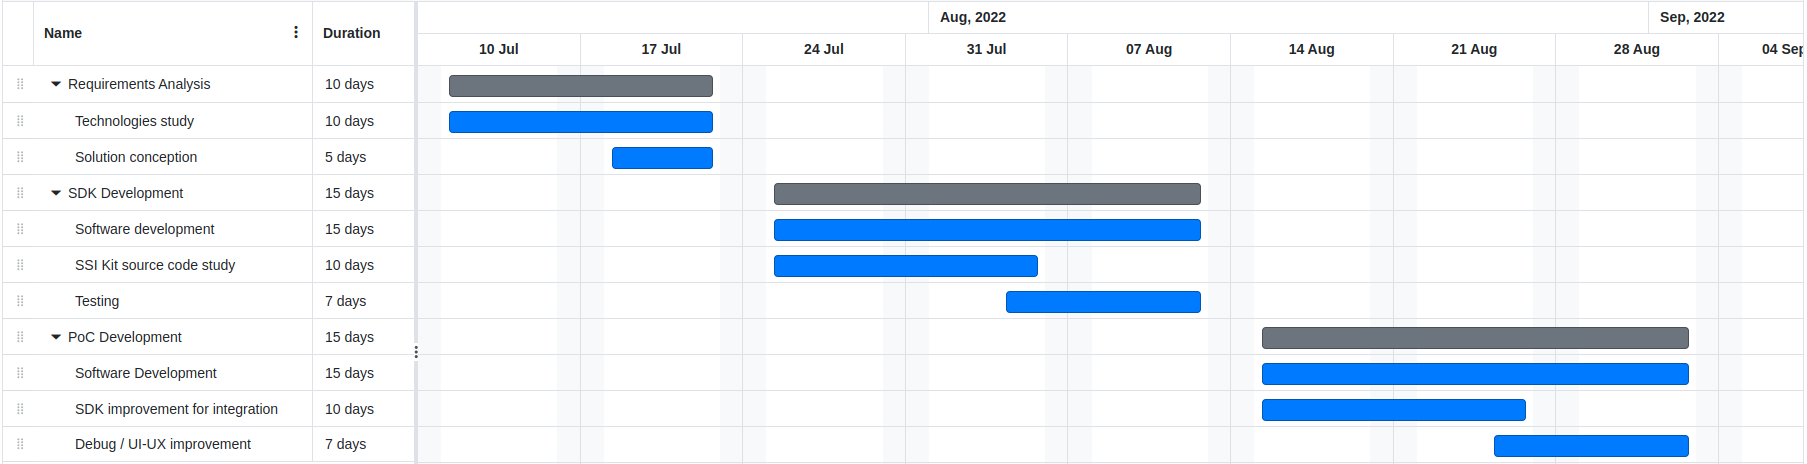
\includegraphics[keepaspectratio = true, width=15cm]{chapter1/internshipGantt.png}
    \captionof{figure}{Internship structure}
\end{center}

% !TEX encoding = UTF-8
% !TEX TS-program = pdflatex
% !TEX root = ../thesis.tex

\chapter{State of the art and technology background}
This chapter presents the pre-concepts needed to comprehend this paper's content fully.
As is understandable from the introduction, they are about Self-Sovereign Identity and 
blockchains. In addition, state of the art will be analyzed to see what has already been
done and what can be improved.
% /*//////////////////////////////////////////////////////////////
%                       TECHNOLOGY CONCEPTS
% //////////////////////////////////////////////////////////////*/
\section{Technology concepts}
This section will explain in detail SSI and blockchain technologies.
\subsection{Self-Sovereign Identity concepts}
Here can be read a brief reprise of what has already been saying about Self-Sovereign 
Identity and a description of its main primitives: VCs, VPs, and DIDs.
\subsubsection{Self-Sovereign Identity}
Self-Sovereign Identity is an approach to digital identity that gives individuals 
control over their data. SSI addresses the difficulty of establishing trust in 
interaction and allows people to interact in the digital world with the same freedom 
and ability to trust as they have in the offline world.
\vspace*{0.3cm}\\
To be trusted, a party in an interaction will present credentials to other parties, 
and those parties can verify that the credentials come from an \textbf{issuer} they trust.
This way, the \textbf{verifier}'s trust in the issuer is transferred to the credential 
\textbf{holder} (or \textbf{prover}). This basic structure of SSI with three participants 
is sometimes called the "triangle of trust.", simply because you need an element of trust
among these entities for them to work together.
\vspace*{0.3cm}\\
While this does not mean that there is a legal partnership or understanding between the 
entities involved, it does mean that each of the entities is willing to examine the 
credibility of the other, and this implicit trust is what constitutes this term.
\begin{center}
    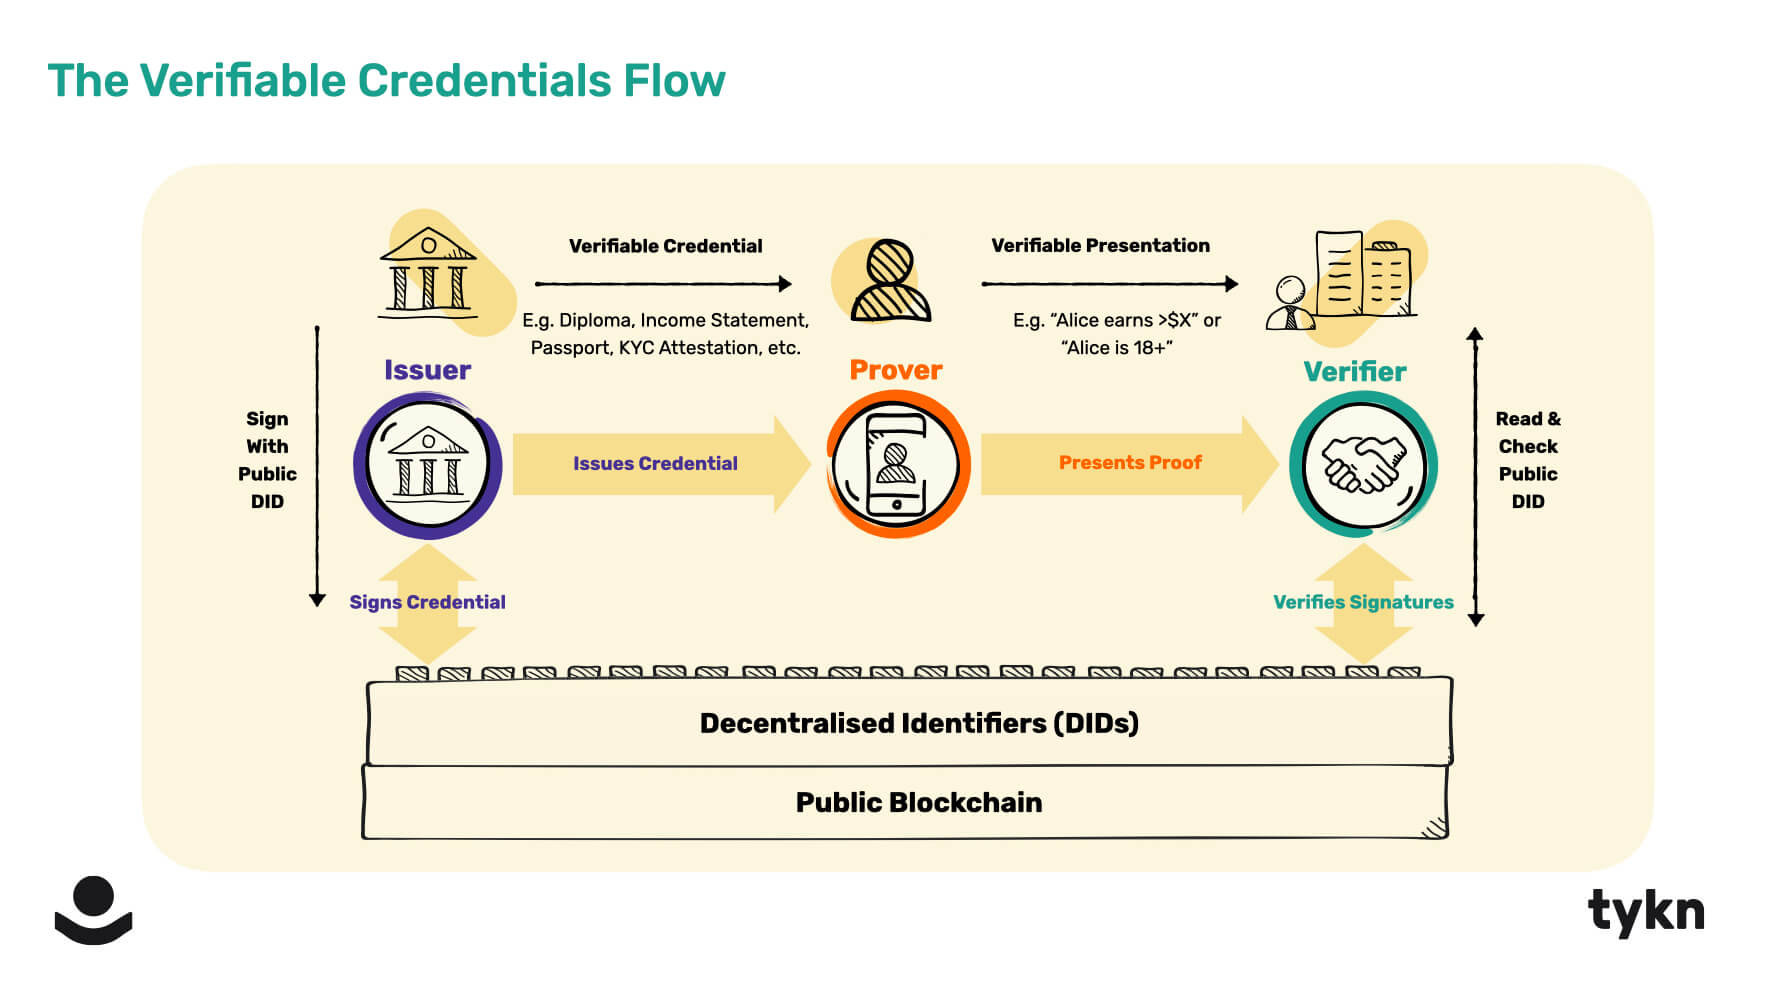
\includegraphics[scale=0.2]{chapter2/triangleTrust2.jpeg}
    \captionof{figure}{The triangle of trust: Prover, Issuer, and Verifier (by Tykn)}
\end{center}
\subsubsection{Verifiable Credential (VC)}
A verifiable credential can represent all of the same information that a physical 
credential represents. The addition of technologies, such as digital signatures, 
makes verifiable credentials more tamper-evident and more trustworthy than their 
physical counterparts.\\
\begin{center}
    \vspace*{-0.5cm}
    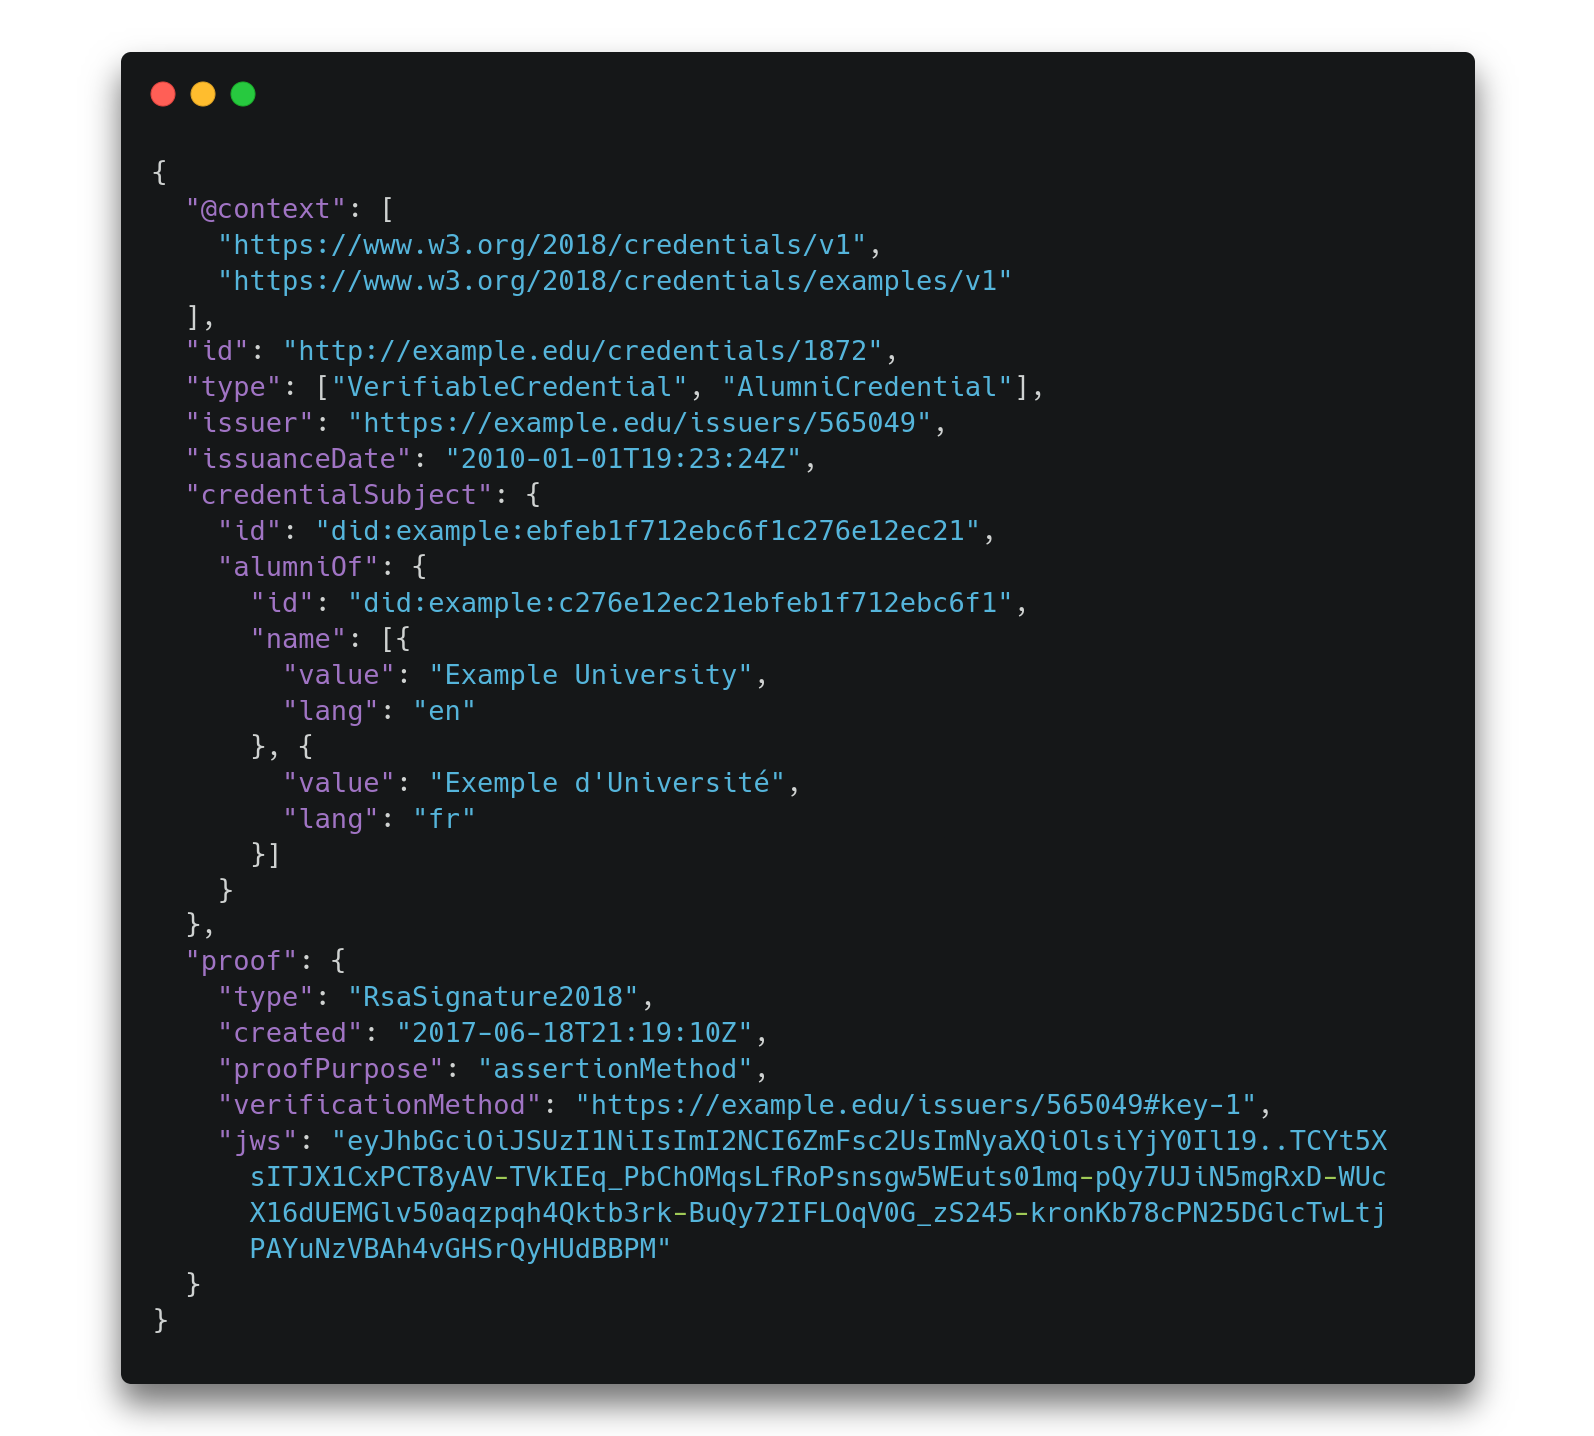
\includegraphics[scale=0.2]{chapter2/exampleVc.png}
    \captionof{figure}{Example of verifiable credential (VC)}
\end{center}
Holders of verifiable credentials can generate verifiable presentations and then share 
these verifiable presentations with verifiers to prove they possess verifiable 
credentials with certain characteristics.\\
Both verifiable credentials and verifiable presentations can be transmitted rapidly, 
making them more convenient than their physical counterparts when trying to establish 
trust at a distance.
The three main components of a VC are:
\begin{enumerate}
    \item \textbf{Metadata}: cryptographically signed by the issuer. It describes the credential
    properties, such as the issuer, the subject, the expiry date and time, a public key 
    to use for verification purposes, the revocation mechanism, and other information;
    \item \textbf{Claims}: a statement made about a subject. Example: “Janice`s date of 
    birth is 01/01/1990.”
    \item \textbf{Proofs}: a proof is data about the identity holder that allows others 
    to verify the source of the data (i.e., the issuer), check that the data belongs to 
    (only) the holder, that the data has not been tampered with, and finally, that the 
    issuer has not revoked the data.
\end{enumerate}

\subsubsection{Verifiable Presentation (VP)}
A verifiable presentation expresses data from one or more verifiable credentials and is 
packaged in such a way that the authorship of the data is verifiable. If verifiable 
credentials are presented directly, they become verifiable presentations. Data formats 
derived from verifiable credentials that are cryptographically verifiable but do not 
themselves contain verifiable credentials might also be verifiable presentations.
\begin{center}
    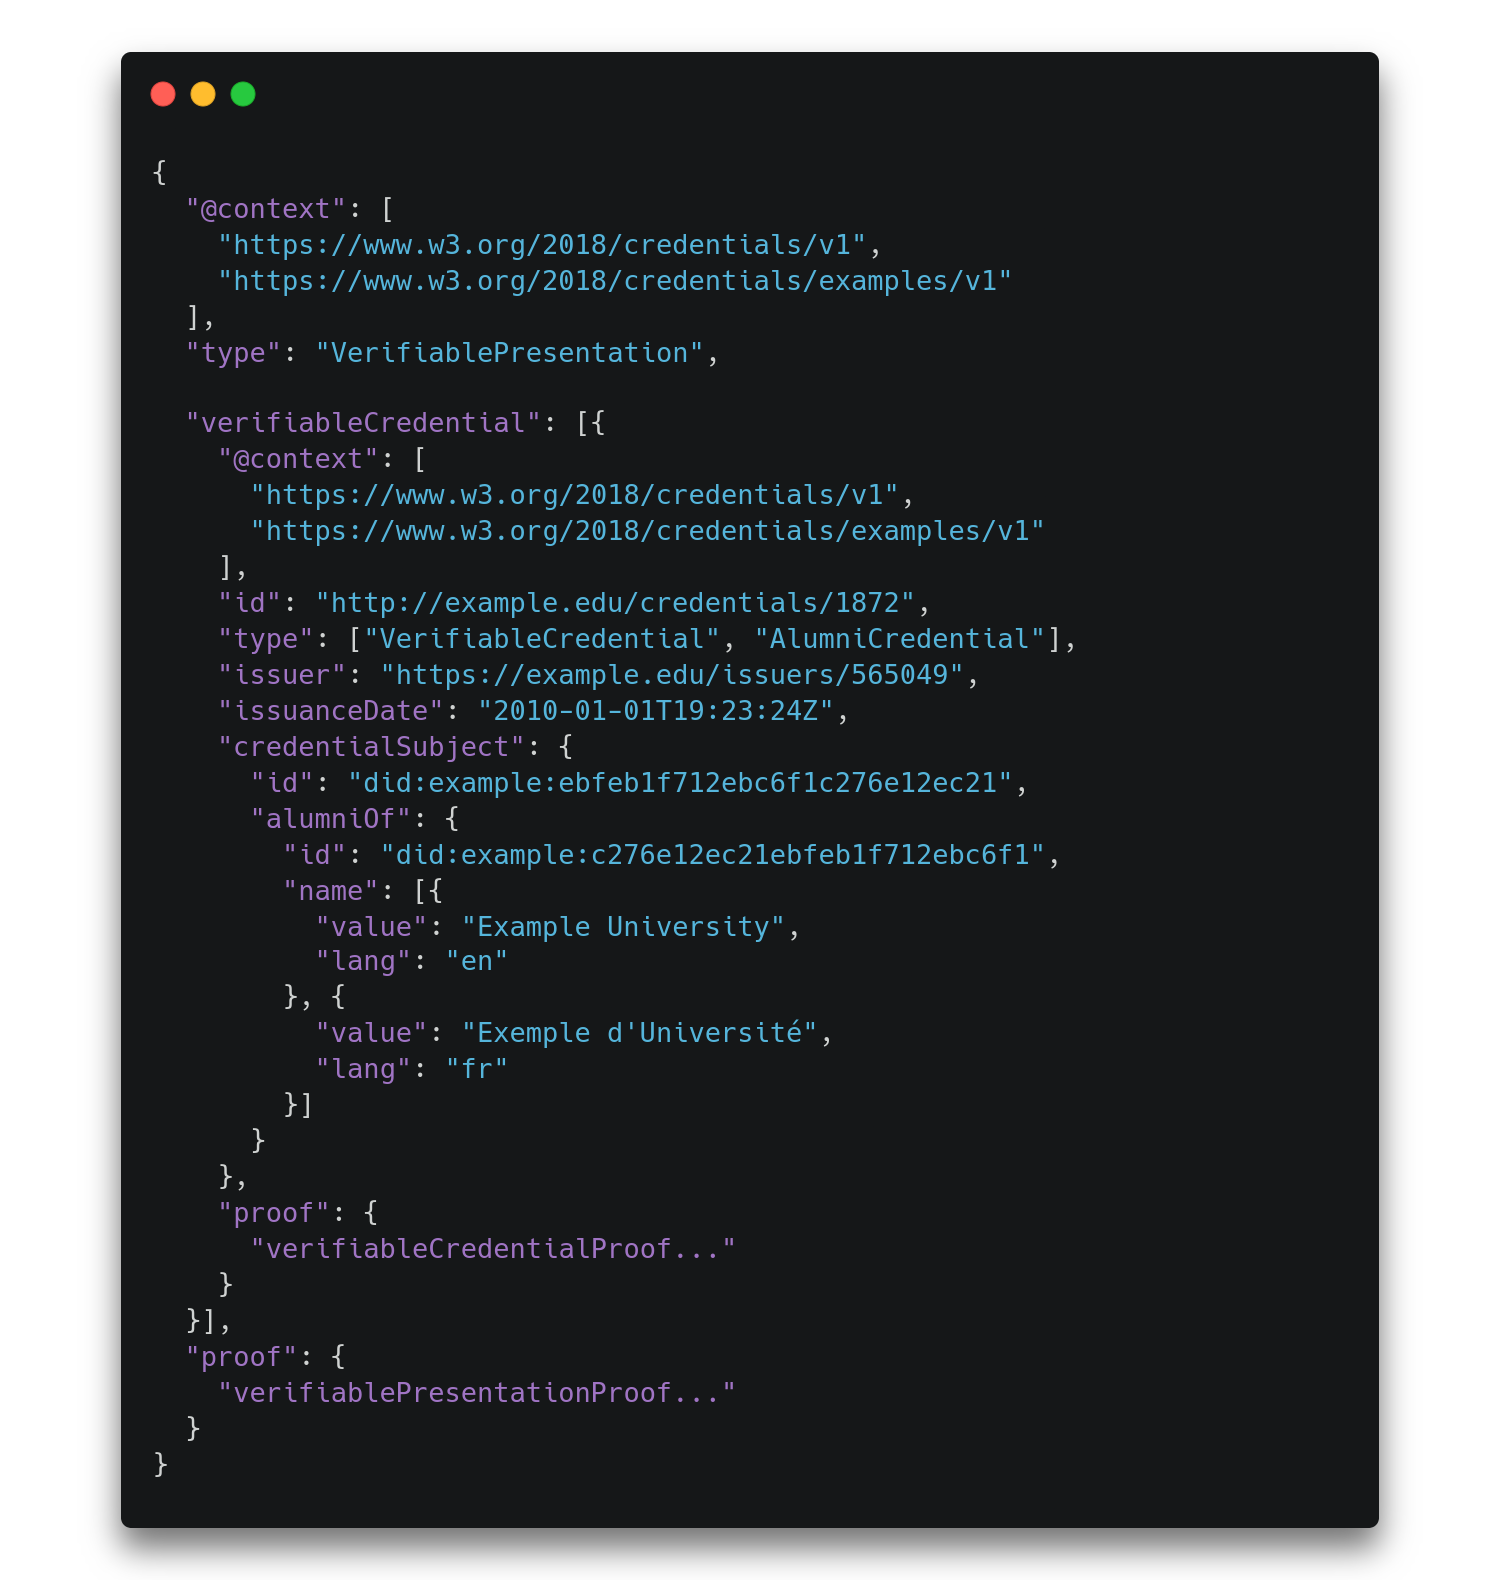
\includegraphics[scale=0.18]{chapter2/exampleVp.png}
    \captionof{figure}{Example of verifiable presentation (VP)}
\end{center}
The data in a presentation is often about the same subject but might have been issued by 
multiple issuers. The aggregation of this information typically expresses an aspect of 
a person, organization, or entity.

\subsubsection{Decentralized Identifier (DID)}
Decentralized identifiers are a new type of identifier that guarantees a verifiable, 
decentralized digital identity. A DID refers to any subject (e.g., a person, an 
organization, a data model, an abstract entity...).\\
DIDs are decoupled from centralized registries, identity providers, and certification 
authorities. Specifically, while other parties can be used to retrieve information 
about a DID, the design allows the controller of a DID to demonstrate control over it 
without requiring permission from other parties.
\begin{figure}[!htb]
    \begin{minipage}{0.48\textwidth}
      \centering
      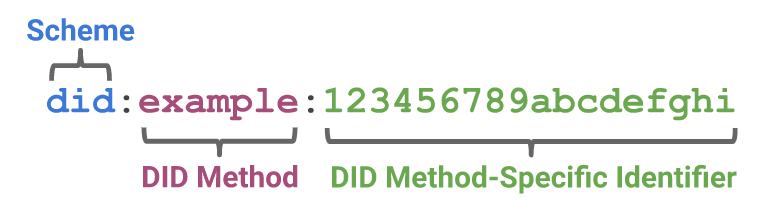
\includegraphics[width=1\linewidth]{chapter2/did1.png}
      \vspace{1.1cm}
      \caption{Example of a DID}
    \end{minipage}\hfill
    \begin{minipage}{0.48\textwidth}
      \centering
      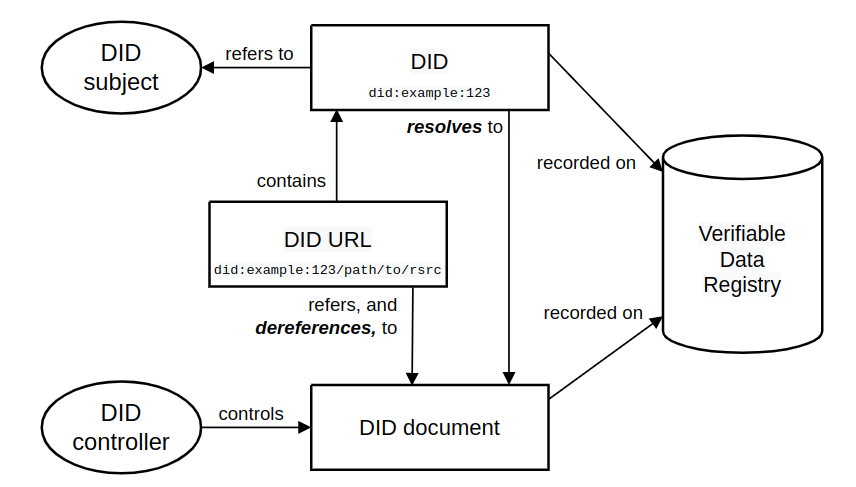
\includegraphics[width=1\linewidth]{chapter2/did2.png}
      \caption{DID architecture overview and basic components relationship}
    \end{minipage}
 \end{figure}
\begin{center}
    \vspace{-0.8cm}
    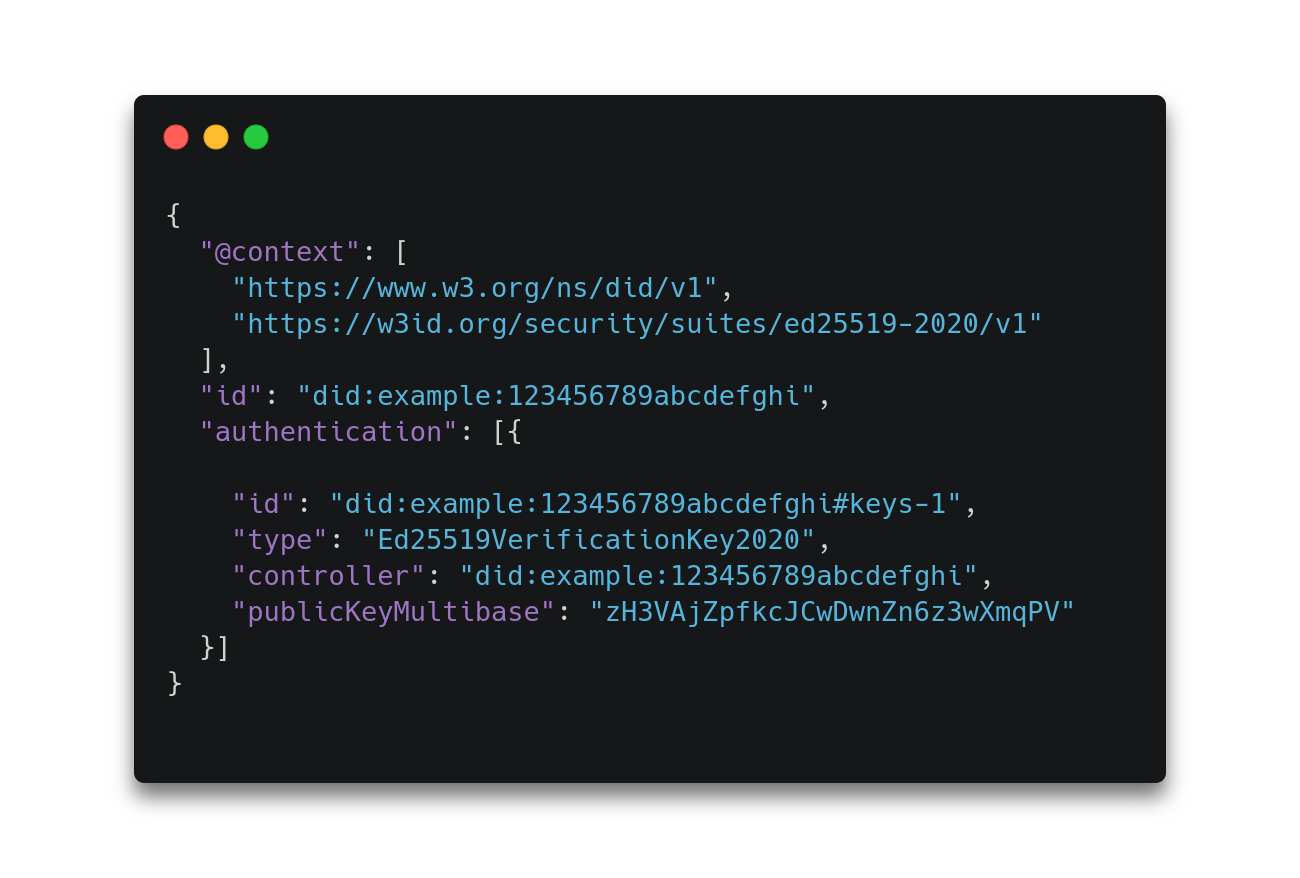
\includegraphics[scale=0.19]{chapter2/didDoc.png}
    \vspace{-0.4cm}
    \captionof{figure}{Example of DID document}
\end{center}
\vspace{0.5cm}
DIDs are Uniform Resource Identifiers (URIs) that associate a DID subject with a DID 
document that enables trusted interactions associated with that subject.
Each DID document may contain encrypted material, verification methods, or services, 
which provide a set of mechanisms that allow a DID controller to demonstrate control 
of the DID. Services enable trusted interactions associated with the subject of the 
DID. A DID may provide the means to return the DID subject itself if the DID subject 
is an information resource such as a data model.\\
A DID is a simple text string consisting of three parts: 1) the DID URI scheme 
identifier \footnote{The formal syntax of a decentralized identifier. The generic 
DID scheme begins with the prefix \textit{did:}.}, 2) the identifier for the DID method
\footnote{A definition of how a specific DID method scheme is implemented.}, and 3) 
the DID method-specific identifier.

\subsubsection{JavaScript Object Notation (JSON)}
The VC, VP and DID document code examples showed above are all in JSON.\\
The JSON is a lightweight data-interchange format. It is easy for humans to read and 
write, and for machines to parse and generate. It is based on a subset of the JavaScript
Programming Language Standard ECMA-262 3rd Edition - December 1999.\\
JSON is built on two structures:
\begin{itemize}
    \item A collection of name/value pairs. In various languages, this is realized as an 
    object, record, struct, dictionary, hash table, keyed list, or associative array.
    \item An ordered list of values. In most languages, this is realized as an array, 
    vector, list, or sequence.
\end{itemize}
These are universal data structures. Virtually all modern programming languages support 
them in one form or another. It makes sense that a data format that is interchangeable 
with programming languages also be based on these structures.
\subsection{Blockchain concepts}
Here we will introduce the main concepts of blockchain technology, essentials to 
understand the PoC development phase and some SDK features.
\subsubsection{Blockchain}
The blockchain is a shared, immutable database structured in the form of a chain of 
blocks, each of which contains a set of information. In essence, blockchains represent 
digital ledgers and perform different functions.
\begin{center}
    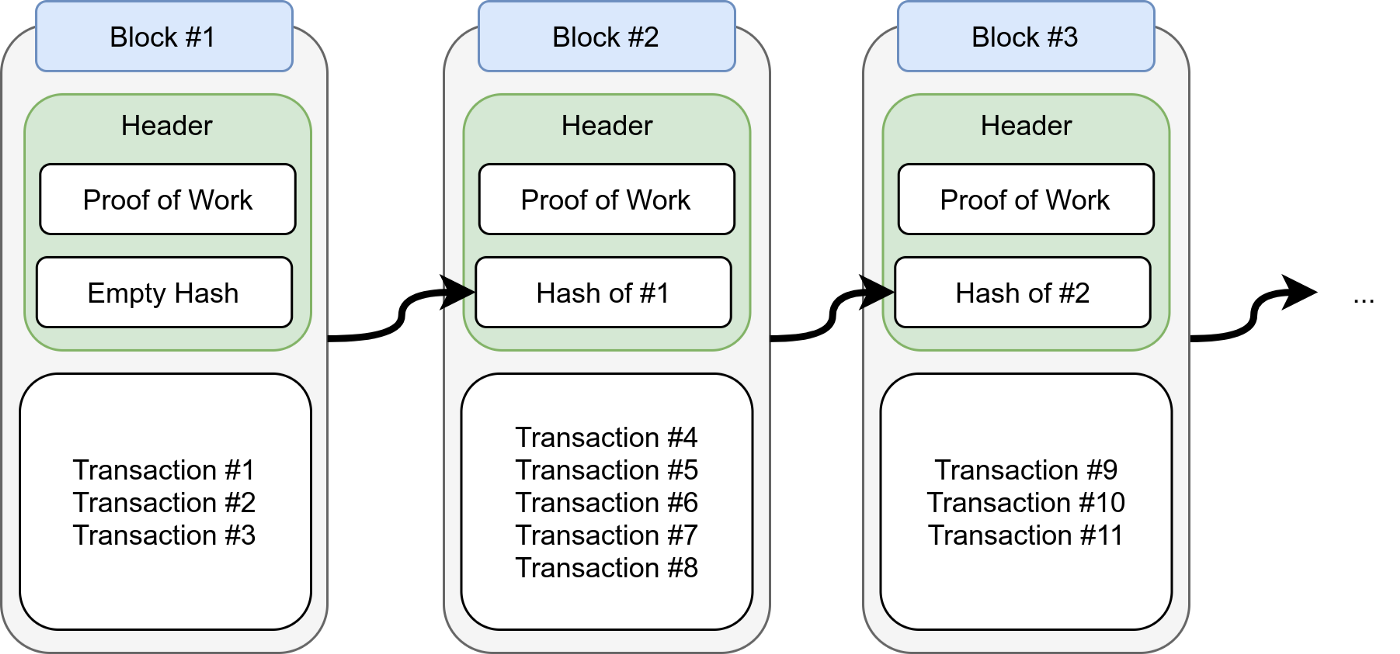
\includegraphics[scale=0.2]{chapter2/blockchain.png}
    \captionof{figure}{Simple blockchain visualization}
\end{center}
Physically it is composed of multiple \textbf{nodes}, i.e., computers that run the software 
(Client) of the blockchain. When a user wants to interact with the blockchain, he 
sends a \textbf{transaction} to one of the nodes. This transaction will then reach a pool with 
all the transactions in the pending state, and the nodes that are dealing with the 
consensus part will take care of updating the state of the blockchain by inserting 
several transactions (meeting certain conditions) within the new \textbf{block} that will
be added to the chain.\\
Its main features are data digitalization, decentralization, disintermediation, 
transfer traceability and programmability, transparency/verifiability, and immutability.
\subsubsection{Permissionless and permissioned blockchains}
We can divide blockchains into two main categories: permissionless and permissioned.
This division is based on the access to the network.
\begin{itemize}
    \item \textbf{Permissionless blockchains} are the most popular model. As its name implies, these 
    networks allow access to anyone and are decentralized and public. Consequently, 
    everyone can run a node or connect to the blockchain.\\
    This accessibility implies a trade-off on speed; these networks are often slower than 
    their permissioned counterparts, with fewer members, and transactions are validated by 
    everyone running a connected node. The primary consensus mechanisms are Proof-of-Work 
    (PoW) and Proof-of-Stake (PoS) \footnote{PoW involves hashing (mining) power, PoS voting 
    (using blockchain coins) power, through validator nodes.}.\\
    What is of most interest in this scenario is that in a permissionless blockchain, 
    everyone can interact, and data is public, so \textbf{preserving privacy becomes difficult}.
    \item \textbf{Permissioned blockchains} are private networks that require permission to
    join. They are usually run by a single organization or a consortium of organizations.\\
    The main advantage of permissioned blockchains is speed. They are faster than
    permissionless blockchains because they have fewer members and transactions are
    validated by a smaller number of nodes. The main consensus mechanisms are Raft and 
    Practical Byzantine Fault Tolerance (PBFT).\\
    The main peculiarity of permissioned blockchains is that they are not decentralized
    and are not public. This means that only a limited number of people can interact with
    the blockchain, and data is not public, so \textbf{privacy can be preserved}.
\end{itemize}

\subsubsection{Ethereum}
Ethereum is a permissionless blockchain, i.e., open to anyone who wants to interact 
with it: the trade-off is the introduction of fees, to be paid every time anyone wants 
to change the state of the Ethereum Virtual Machine (EVM), to mitigate the problems 
that the permissionless factor introduces (e.g., transaction spam). In the read-only 
case, no fee needs to be paid. Anyone can then view what is happening in the blockchain 
and, more importantly, use it. To do so, a user has to generate a \textbf{wallet} (i.e.,
an address in the blockchain), transfer some funds to it from outside \footnote{Usually
from a centralized exchange, where cryptoc-urrencies can be traded for fiat currencies
like EUR or USD, or from another blockchain.} so that fees can be paid, and start 
interacting with the decentralized applications that are already developed or transfer 
funds to other wallets. In fact, one of the main features of Ethereum is \textbf{smart 
contracts}: they are programs that run on the Ethereum blockchain. They are a collection 
of code (functions) and data (state) that resides at a specific address on the 
Ethereum blockchain.
\subsubsection{Hyperledger}
Hyperledger Foundation is a nonprofit organization that combines all the resources and 
infrastructure needed to ensure thriving and stable ecosystems around open-source 
software blockchain projects.\\
Hyperledger Foundation staff are part of the larger \textbf{Linux Foundation} team with
years of experience providing management services for programs for open-source projects.
\subsubsection{Hyperledger Besu}
Hyperledger Besu is an Ethereum client designed to be enterprise-friendly for use cases 
of public and private permissioned networks, which require secure transaction processing
and high performance.\\
The Besu blockchain, therefore, is EVM compatible: from the perspective of developers 
and users, interaction with it will be very similar to interaction with Ethereum. It 
places particular emphasis, however, on \textbf{privacy and permissioning} features; in fact, 
only those who are authorized (i.e., those who own a connected node) can interact with 
the system, which is the primary difference from Ethereum.
\begin{figure}[!htb]
    \begin{minipage}{0.48\textwidth}
        \centering
        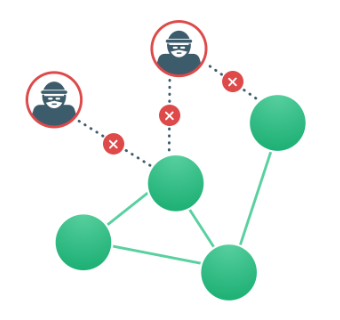
\includegraphics[width=.77\linewidth]{chapter2/privacyEsterno.png}
        \caption{Only allowed users can participate in the network}
    \end{minipage}\hfill
    \begin{minipage}{0.48\textwidth}
        \centering
        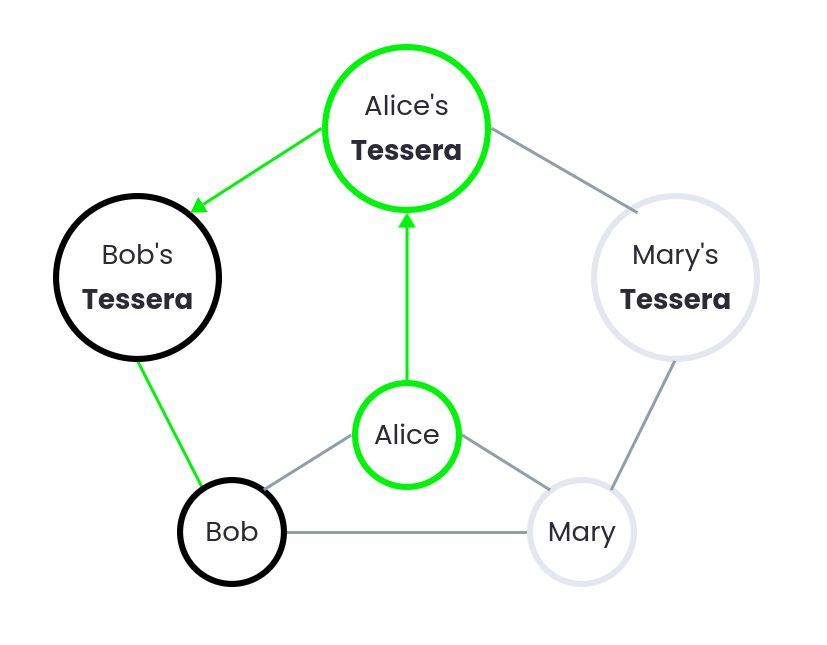
\includegraphics[width=1\linewidth]{chapter2/privacyInterno.png}
        \caption{Mary cannot see the private transaction sent from Alice to Bob}
    \end{minipage}
\end{figure}
\begin{figure}[!htb]
    \begin{minipage}{0.48\textwidth}
        \centering
        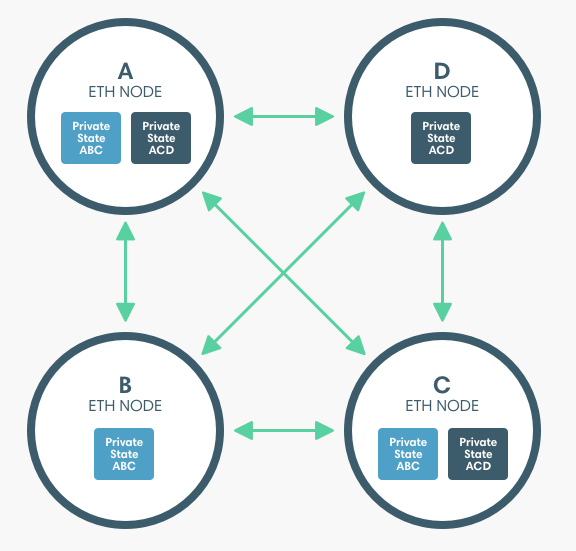
\includegraphics[width=.77\linewidth]{chapter2/privacyGroups.png}
        \caption{Restricted visibility of two Privacy Groups (light blue and blue)}
    \end{minipage}\hfill
    \begin{minipage}{0.48\textwidth}
        \centering
        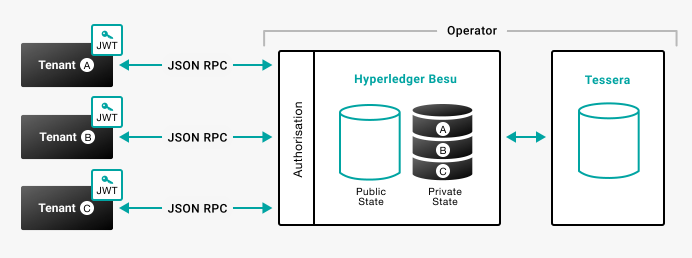
\includegraphics[width=1\linewidth]{chapter2/multiTenant.png}
        \caption{Besu and Tessera pair nodes administrator can give access to other Tenants, i.e., users.}
    \end{minipage}
\end{figure}\\
Privacy is enabled both externally to the network and internally: through private 
transactions, not all nodes can access certain information, and nodes that want to 
take advantage of private transactions must have an associated \textbf{Tessera} node, which 
will take care of the cryptographic part.\\
Even \textbf{Privacy Groups} can be created: those who do not belong to the group cannot access 
particular data. In addition, another interesting feature is that of Multi-Tenant 
management: multiple participants can use the same Besu and Tessera node through a 
dedicated user system.

\subsubsection{Hyperledger Fabric}
Hyperledger Fabric is an enterprise-grade, proven, and open distributed ledger 
platform (DLT). It provides advanced privacy controls so that only the shareable 
data is transmitted among network participants, known as "authorized".\\
It offers a modular architecture that makes available components (mechanism for 
consensus, services for joining and managing blockchain members) that can be activated
within a blockchain with plug-and-play logic. It can be said to be very similar to 
Besu (also a permissioned and privacy-oriented), with the big difference being that 
it is not EVM compatible so the smart contracts will be written in languages such as 
Java and Go instead of Solidity.
\subsection{Libraries and Stack involved}
\subsubsection{EBSI}
\subsubsection{walt.id SSI Kit}

% /*//////////////////////////////////////////////////////////////
%                        STATE OF THE ART
% //////////////////////////////////////////////////////////////*/
\section{State of the art}

% !TEX encoding = UTF-8
% !TEX TS-program = pdflatex
% !TEX root = ../thesis.tex

\chapter{Solution}
Now we discuss the path we decided to take, how we developed the software, 
and the technologies we leveraged. Then, we outline the final achievements 
and what can be done to enhance the PoC potential.
\section{Solution proposal}
After the conducted analysis in the first two weeks, we concluded that building a 
new system from zero would have needed too much time and effort, and especially would 
have required specific advanced skills we did not have.\\
First, we recall that we are building agents for verifiable credentials interaction. 
In a full stack product, our solution is placed between the users, who use secure 
communication protocols\footnote{For example, OAuth or OIDC, as can be seen in the
Figure 3.1},  and VDRs\footnote{For example EBSI, Sovrin or IBSI, blockchain used for
SSI purposes}, which store the DIDs, credentials schema, verification policies, 
and more.
\begin{center}
    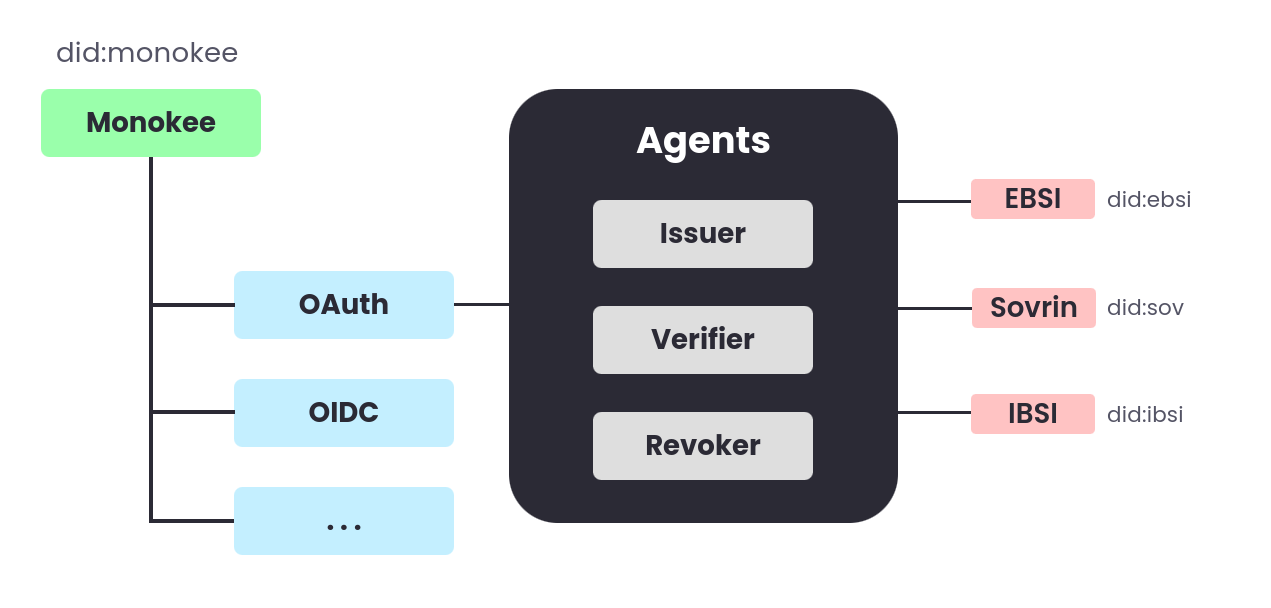
\includegraphics[scale=0.28]{chapter3/problem_schema.png}
    \captionof{figure}{Monokee ideal scenario}
\end{center}
\vspace*{0.5cm}
Figure 3.1 shows the ideal scenario, where Monokee will have its own DID method
(did:monokee), through which will be generated identifiers that will hide (at least,
as far as the user is concerned) the blockchain where it is located.
\vspace*{0.3cm}\\
The final software structure has three main components:
\begin{itemize}
    \item \textbf{Frontend}: it allows the user to interact with the system's core 
    functionalities and serves as an interface for every SSI Kit SDK function.
    \item \textbf{Backend}: it is needed for security, as we will analyze 
    further, and for cryptographic functions that the frontend could not execute.
    \item \textbf{SSI Kit SDK}: it exposes all the SSI functionalities, and enables 
    the user to create keys and DIDs, issue VC, present them as VPs, and more.
    \item \textbf{Smart Contracts}: for what concerns SSI Kit integration, the 
    contracts serve as trusted verifiers and verification results register. Some 
    contracts emit ERC-721 tokens, which let the user request the diploma, but they 
    will not be discussed here.
\end{itemize}
Figure 3.2 shows the system final architecture visualization.
\begin{center}
    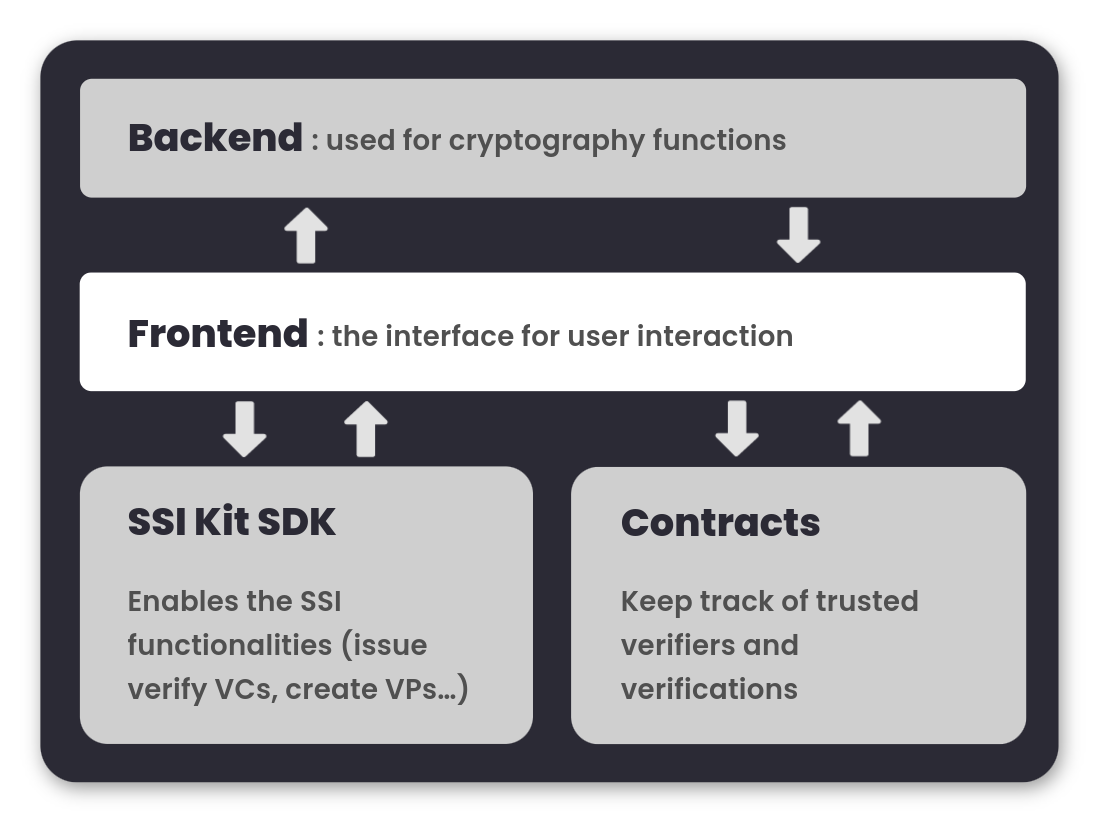
\includegraphics[scale=0.28]{chapter3/structure.png}
    \captionof{figure}{Solution visual representation}
    \label{fig:structure}
\end{center}

\clearpage
\section{Solution development}
In the following sections, we discuss the technologies we used to build the
solution, and we explain the main functionalities of the system.
\subsection{Technologies and Tools}
Before explaining the solution, we list the languages and tools we leveraged to develop it,
for both SSI Kit SDK and PoC.

\subsubsection{Common tools and languages}
\begin{itemize}
    \setlength\itemsep{-0.1em}
    \item \texttt{Typescript}: a strongly typed programming language that builds 
    on JavaScript. It was chosen because the other Monokee's modules were in 
    Typescript, so it would have been easier for the team to integrate. Also, it is 
    very convenient for its strongly typed nature;
    \item \texttt{JSON}: as already covered in \hyperref[subsubsec:json]{Chapter 2}, 
    \texttt{JSON} is a lightweight data-interchange format. It has been extensively used,
    mainly for credentials representation and API calls;
    \item \texttt{Node.js}: a JavaScript runtime built on Chrome's V8 JavaScript
    engine. It has been used for code execution;
    \item \texttt{npm}: a package manager for the JavaScript programming language.
    It has been used to manage the dependencies of the projects;
    \item \texttt{Git}: a free and open-source distributed version control system
    used for tracking and collaboration purposes;
    \item \texttt{Visual Studio Code}: the Integrated Development Environment (IDE)
    we have used for the solution development.
\end{itemize}

\subsubsection[SSI Kit SDK]{SSI Kit SDK\footnote{\texttt{uuid}, \texttt{rfc4648}, 
\texttt{sha256}, and \texttt{nacl} have been used just to generate tokens used for 
credentials revocation, as can be reed \hyperref[method:isRevoked]{here}}}

\begin{itemize}
    \setlength\itemsep{-0.1em}
    \item \texttt{jest}: a JavaScript testing framework. It has been used to test
    the SSI Kit SDK components;
    \item \texttt{waltid-ssikit}: the library written in Kotlin/Java that provides 
    the SSI functionalities set. The developed SDK is a Typescript wrapper of this 
    library;
    \item \texttt{axios}: a promise-based HTTP client for the browser and node.js,
    used to make API calls to waltid-ssikit;
    \item \texttt{uuid}: a library used to generate RFC-compliant Universally Unique
    Identifiers (UUIDs);
    \item \texttt{rfc4648}: a library used to encode and decode data in Base32 format;
    \item \texttt{sha256}: a library used to generate SHA-256 hashes;
    \item \texttt{nacl}: a library used to decode UTF8 \texttt{strings};
\end{itemize}

\subsubsection{Frontend}
\begin{itemize}
    \setlength\itemsep{-0.1em}
    \item \texttt{React.js}: a JavaScript library for building user interfaces. It
    has been used to build the frontend;
    \item \texttt{Chakra-UI}: a simple, modular and accessible components library,
    used with \texttt{React.js} to build the frontend.
    \item \texttt{ethers}: a library used to interact with Ethereum Virtual
    Machine compatible blockchains;
    \item \texttt{wagmi}: a collection of React Hooks containing everything needed
    to start working with Ethereum; it has been used to interact with the smart
    contracts;
    \item \texttt{RainbowKit}: RainbowKit is a React library that makes it easy to 
    add the wallet connection, e.g., for Metamask integration.
    \item \texttt{GraphQL}: the query language used by The Graph;
    \item \texttt{ssikit-sdk}: the developed Typescript SDK used to interact with 
    the SSI Kit library.
    \item \texttt{The Graph}: a decentralized protocol for indexing and querying
    data from blockchains, starting with Ethereum. It makes it possible to query 
    data that is difficult to query directly. It has been used to query The
    deployed smart contracts.
    \item \texttt{smart contracts suite}: a collection of smart contracts used to
    register the verifications and the verification results on-chain.
\end{itemize}

\subsubsection{Backend}
\begin{itemize}
    \setlength\itemsep{-0.1em}
    \item \texttt{Express.js}: a web application framework for Node.js. It has been
    used to build the backend, where the cryptographic functions are executed; the frontend
    calls them through API calls;
    \item \texttt{ssikit-sdk}: the developed Typescript SDK used to interact with
    the SSI Kit library.
    \item \texttt{jose}: a library used to encode and decode \texttt{JSON} Web Tokens (JWTs),
    which have been used to represent private and public keys;
    \item \texttt{nodemon}: a tool that automatically restarts the node application
    when file changes in the directory are detected.
\end{itemize}

\subsection{SSI Kit SDK development}
In this section we describe the SSI Kit SDK development, which is the core of the
solution. The SDK is a Typescript wrapper of the waltid-ssikit library, which is
written in Kotlin/Java. The SDK exposes all the functionalities of the library,
and it is used by the frontend and the backend to interact with the SSI Kit.

\subsubsection{walt.id SSI Kit}
First, we need to know how to interact with it to understand how to build the SDK.
The kit gives us three options:
\begin{itemize}
    \item \textbf{CLI Tool}: it offers a rich set of commands to run the entire functionality 
    the SSI Kit provides. The CLI tool can be used by running the Docker container or
    the executable by the local build.
    \item \textbf{Dependency (JVM)}: it can be used directly as JVM-dependency via Maven or 
    Gradle.
    \item \textbf{REST API}: it can be run as a service, so an application can access its 
    functionalities via REST API.
\end{itemize}
As we decided to build a Typescript SDK, the REST API is the most convenient way 
to access the kit's functionalities: if we chose CLI, every time we call an SDK 
method,  we should have fired a shell command translating the method execution, and 
it would be the most uncomfortable option. The Dependency option, in addition, is 
immediately discardable as we do not use Maven or Gradle (the application is not 
Java/Kotlin based).\\
The REST API service, instead, is very immediate to integrate into an SDK.
In fact, we previously defined the SDK as a "wrapper" because the SDK methods (at 
least, the great majority) forward their execution as an API call to the underlying 
kit. This makes the interaction with the kit a lot easier for Javascript/Typescript 
application based.
\vspace*{0.3cm}\\
Let us now describe how the SSI Kit API is structured to explain later the choices 
made for the SDK development.
\paragraph{Structure.}
The API is divided in five main components:
\begin{itemize}
    \item \textbf{Signatory}: the component that manages the issuing and
    revocation of verifiable credentials. Also, it can list the credential templates
    used to issue them;
    \item \textbf{Custodian}: gives a CRUD interface for keys, DIDs and credentials.
    Here also can be generated VPs;
    \item \textbf{Auditor}: enables the user to manage verification policies,
    and verify any verifiable credential or presentation;
    \item \textbf{ESSIF}: enables the user to interact with EBSI blockchain (e.g.,
    register a DID);
    \item \textbf{Bonus: Core API}: It is a set of functionalities chosen from the 
    above components. However, the team writes in the documentation that it will not 
    be maintained. For this reason we decided to not build a class for this component.
\end{itemize}
Assuming this, we can say it could be a good idea to build a class for each component 
to organize the SDK better and separate the code.

\subsubsection{SSI Kit Typescript SDK}
After analyzing the SSI Kit structure, we can describe how we developed the SDK.
As stated above, we decided to build a class for each SSI Kit component to modularize 
the SDK. In every class, we put a method corresponding to an API call.\\
For API calls, we use Axios, through which we perform a call in each SDK method. So 
a good thing to do is to create a generalized function, called in every method, 
without writing the same code where possible.
\vspace{0.3cm}\\
Figure 3.3 shows a snippet of the \texttt{callAPI} function, which is used to perform
the API calls.
\begin{center}
    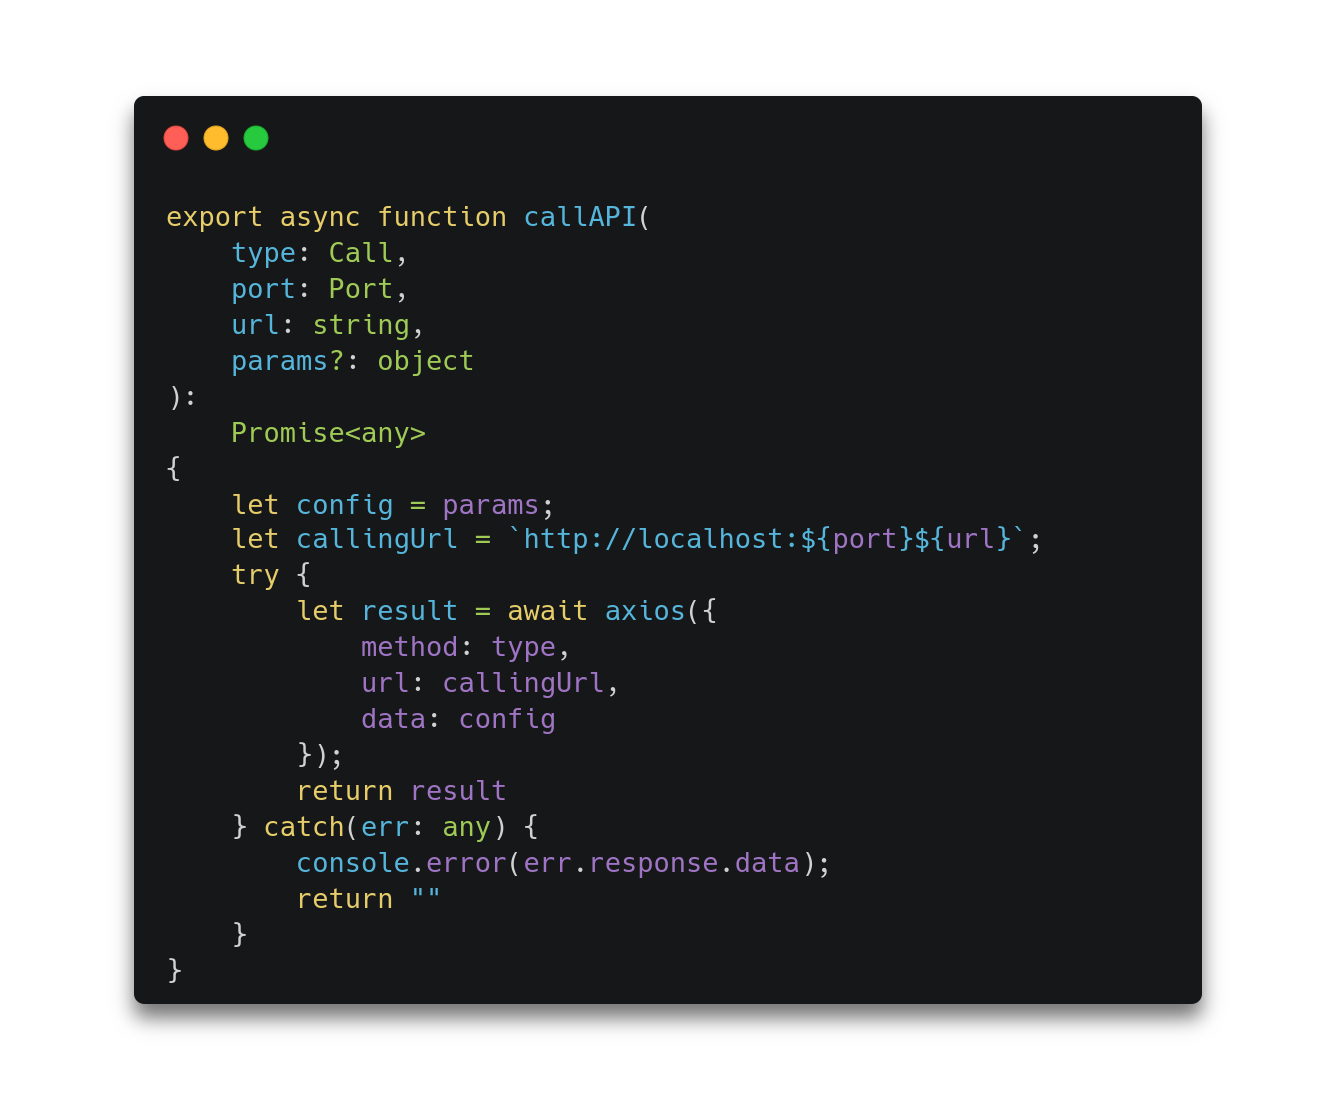
\includegraphics[scale=0.24]{chapter3/callAPIfunction.png}
    \vspace{-0.5cm}
    \captionof{figure}{Snippet of the callAPI function.}
    \label{fig:callAPI}
\end{center}
\vspace{0.5cm}
As input, it takes four parameters:
\begin{itemize}
    \item \texttt{type}: the HTTP method to use; it can be \texttt{"GET"}, \texttt{"POST"},
    \texttt{"PUT"} or \texttt{"DELETE"};
    \item \texttt{port}: the SSI Kit service needs to be run to use the SDK. It then makes
    available four ports, which are used to access the different components of the
    SSI Kit. The \texttt{port} parameter is used to specify which port to use; it can
    be 
    \begin{itemize}
        \item \texttt{7001} (Signatory);
        \item \texttt{7002} (Custodian);
        \item \texttt{7003} (Auditor);
        \item \texttt{7004} (ESSIF);
        \item \texttt{8080} (Universal Resolver);
    \end{itemize}
    \item \texttt{url}: the URL of the API call (e.g., \texttt{"/v1/verify"} to call
    the credentials verification method of the SSI Kit);
    \item \texttt{params}: this is an optional parameter, which is used to pass
    additional info to the call if needed.
\end{itemize}
The return type is generic, as there are many types of results (keys, DIDs, VCs,
booleans, and more). Also, it can be seen that the two parameters \texttt{type} and
\texttt{port} have user defined types. These types and the \texttt{apiCall} function 
can be found inside the file \texttt{utils.ts}, which is a collection of types, 
functions and interfaces used by the SDK, as we analyze in the next section.
\vspace{0.3cm}\\
For the most input/output object parameters of the API calls, we created interfaces
to type them. This is useful to have a better understanding of the parameters, to 
avoid errors and to facilitate the use of the SDK.\\
For verifiable credentials, we did not, as their structure may change from istance
to istance. We simply treat them as \texttt{JSON} objects.\\
We could leave everything as a \texttt{JSON} object, but we decided to create interfaces for
the most important objects. Leaving them as \texttt{JSON} objects would have been a bad idea,
as it would have been difficult to understand what the parameters are and what they
do. The only pro would have been to avoid the creation of interfaces, but we think
that the cons are more important.

\paragraph{Structure.}
The SDK is composed of five main classes. Four are the classes corresponding to the 
four previously described components of the SSI Kit, and the fifth is the one dedicated
to the Universal Resolver. Other than this, the SDK offers a \texttt{utils.ts} file.
\vspace{0.3cm}\\
The SSI Kit SDK splits into three main folders:
\begin{itemize}
    \item \texttt{core}: it contains the main classes of the SDK, which are the
    ones that interact with the SSI Kit API; it also contains the \texttt{utils.ts}
    file, which is a collection of types, functions, and interfaces used by the SDK,
    and the \texttt{lib.ts} file, which contains two functions that perform multiple
    SDK calls (e.g., \texttt{registerDIDOnEBSI} which performs the entire onboarding
    procedure of a DID in the EBSI blockchain);
    \item \texttt{interfaces}: it contains the interfaces used by the four SSI Kit
    class implementations;
    \item \texttt{tests}: it contains the tests of the SDK.
\end{itemize}
Everything (function, type, interface) with the \texttt{export} declaration gets exported by the \texttt{index.ts}
file, which is the entry point of the SDK.

\paragraph{Functionalities.}
After examining the SDK structure, the choices we made, and some technical detail, we can now 
fully explain its functionalities.
\begin{itemize}
    \setlength{\itemsep}{1cm}

    \item \textbf{Signatory}: this class serves as the issuer component in our
    SSI model. It implements five methods:
    \begin{itemize}
        \setlength{\itemsep}{0.4cm}
        \item[] \code{issueCredential}: issues a verifiable credential;
        \begin{itemize}
            \item \textbf{Params}: \texttt{IssueCredentialRequest}, which is an object where 
            it is specified the template ID (chosen by those provided by the SSI Kit), the
            credential data and the proof configuration;
            \item \textbf{Returns}: a W3C Verifiable Credential in \texttt{JSON} format.
        \end{itemize}
        \item[] \code{getVCTemplateIDs}: returns the IDs of all the SDK templates;
        \begin{itemize}
            \item \textbf{Returns}: an \texttt{array} of \texttt{strings}, where each \texttt{string} is a template ID
            (e.g., \texttt{"UniversityDegree"}); these templates are usable in the
            \texttt{issueCredential} method.
        \end{itemize}
        \item[] \code{getVCTemplate}: it returns a specific template;
        \begin{itemize}
            \item \textbf{Params}: the \texttt{templateId} \texttt{string};
            \item \textbf{Returns}: a verifiable credential template in \texttt{JSON} format.
        \end{itemize}
        \item[] \code{isRevoked}: checks if a verifiable credential is revoked;
        \label{method:isRevoked}
        \begin{itemize}
            \item \textbf{Params}: the corresponding \texttt{publicRevocationToken};
            \item \textbf{Returns}: the result of the check, which is an object with the
            fields \texttt{revoked} (boolean) and \texttt{token} (\texttt{string});
            \item \textbf{Notes}: the \texttt{publicRevocationToken} is findable
            inside the \texttt{\seqsplit{credentialStatus}} field of the VC. When an issuer issues
            a VC, the SDK generates a \texttt{private} and a \texttt{public} revocation token. 
            The \texttt{private} has to be saved by the issuer, and can be used to revoke 
            the credential. The \texttt{public} one is included in the VC, and everyone can 
            use it to check if the VC has been revoked or not. Figure 3.4 shows the functions
            used to generate the revocation tokens (in 
            \texttt{utils.ts}). The \texttt{baseToken} is the private one, and is a 
            concatenation of two random UUIDs. The \texttt{publicToken} is the derived by
            the \texttt{baseToken} in this manner: 
            \texttt{base32(sha256(baseToken)).replaceAll("=", "").}
        \end{itemize}
        \begin{center}
            \hspace{-1.5cm}
            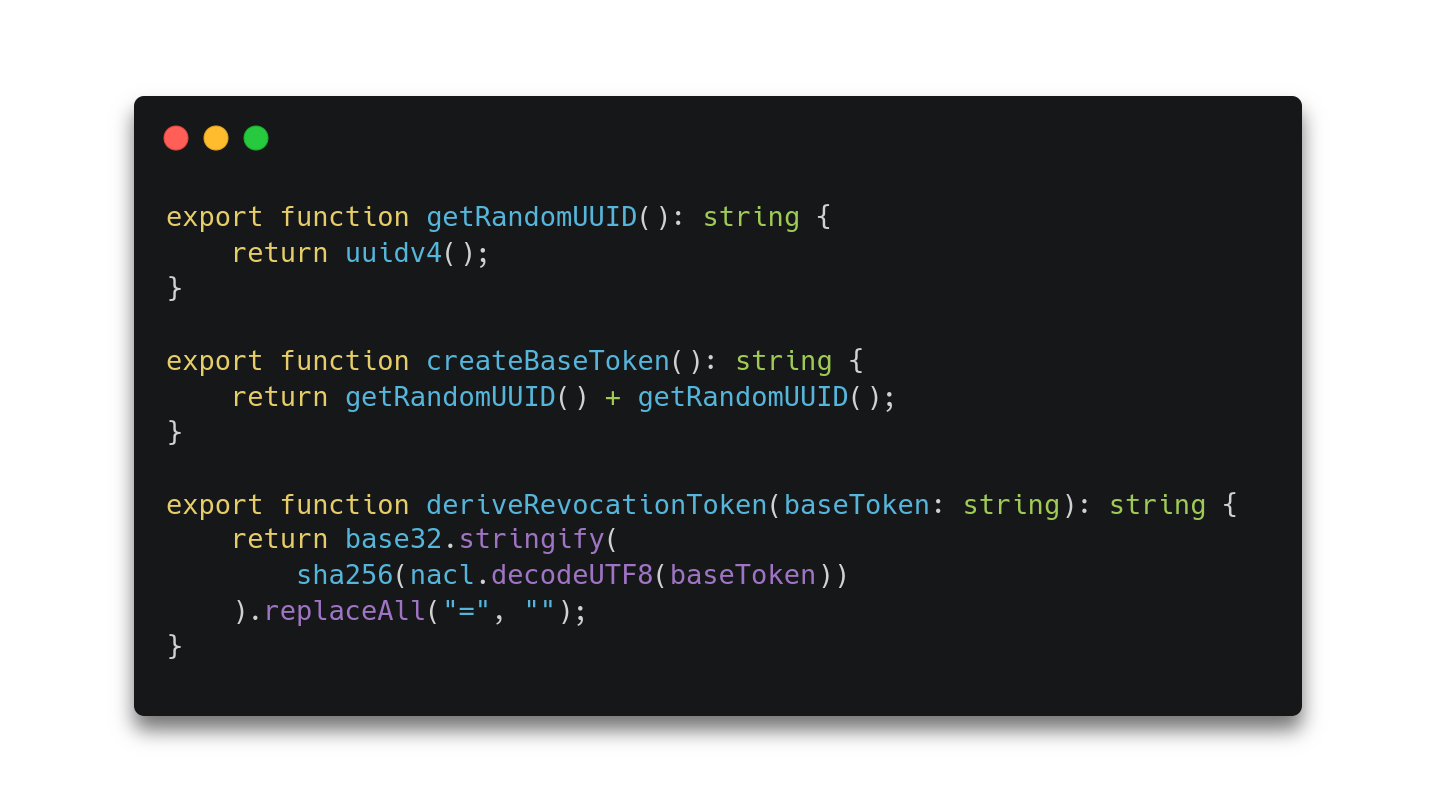
\includegraphics[scale=0.22]{chapter3/revocation.png}
            \vspace{-0.3cm}
            \captionof{figure}{Revocation tokens functions snippet}
        \end{center}
        \vspace{0.3cm}
        \item[] \code{revokeCredential}: revokes a verifiable credential;
        \begin{itemize}
            \item \textbf{Params}: the \texttt{privateRevocationToken}, owned only by the 
            issuer of that VC;
            \item \textbf{Returns}: the revocation result, which is a \texttt{boolean} (if
            \texttt{false}, something went wrong during the process).
        \end{itemize}
    \end{itemize}

    \item \textbf{Custodian}: this class serves as the holder component in our
    SSI model. It implements eighteen methods, and manages keys, DIDs and credentials:
    \begin{itemize}
        \setlength{\itemsep}{0.4cm}
        \item[] \code{getKeys}: gets the keys in the holders's wallet;
        \begin{itemize}
            \item \textbf{Returns}: an \texttt{array} of \texttt{Key} objects, which are the keys
            owned by the holder.
        \end{itemize}
        \item[] \code{getKey}: gets a specific key in the holder's wallet;
        \begin{itemize}
            \item \textbf{Params}: the \texttt{keyId} \texttt{string}, which is the key identifier;
            \item \textbf{Returns}: the corresponding \texttt{Key} object.
        \end{itemize}
        \item[] \code{generateKey}: generates a new key;
        \begin{itemize}
            \item \textbf{Params}: the \texttt{keyAlgorithm} \texttt{string}, that specifies
            the algorithm used to generate the key; the supported algorithms are 
            \texttt{RSA}, \texttt{EdDSA\_Ed25519} and \texttt{EdDSA\_Secp256k1};
            \item \textbf{Returns}: the generated \texttt{Key} object.
        \end{itemize}
        \item[] \code{deleteKey}: deletes a key from the holder's wallet;
        \begin{itemize}
            \item \textbf{Params}: the \texttt{key} parameter, which can be the \texttt{keyId}
            \texttt{string} or the \texttt{Key} object;
            \item \textbf{Returns}: the result of the deletion, which is a \texttt{boolean}.
        \end{itemize}
        \item[] \code{exportKey}: exports a key (private or public) in the desired format;
        \begin{itemize}
            \item \textbf{Params}: the \texttt{key} parameter (\texttt{id string} or \texttt{Key} object),
            the \texttt{format}, which can be \texttt{JWK} or \texttt{PEM}, and \texttt{exportPrivate}
            (if \texttt{true}, the private key is exported, otherwise the public one);
            \item \textbf{Returns}: the exported key in \texttt{JSON} format.
        \end{itemize}
        \item[] \code{importKey}: imports a key in the holder's wallet;
        \begin{itemize}
            \item \textbf{Params}: the \texttt{formattedKey} parameter (\texttt{JWK} or \texttt{PEM} format),
            \item \textbf{Returns}: the \texttt{keyId} of the imported key.
        \end{itemize}
        \item[] \code{getDIDs}: gets the DIDs owned by the holder;
        \begin{itemize}
            \item \textbf{Returns}: an \texttt{array} of \texttt{DID strings}.
        \end{itemize}
        \item[] \code{getDID}: gets a specific DID owned by the holder, from local storage;
        \begin{itemize}
            \item \textbf{Params}: the \texttt{did string};
            \item \textbf{Returns}: the corresponding DID \texttt{JSON} with related metadata
            (e.g., \texttt{verificationMethod}, used to verify the DID signature).
        \end{itemize}
        \item[] \code{createDID}: creates a new DID;
        \begin{itemize}
            \item \textbf{Params}: the \texttt{method} (\texttt{key}, \texttt{web} or \texttt{ebsi}),
            the \texttt{key} (\texttt{object} or id \texttt{string}) used to generate the DID, and
            two optionals (for \texttt{web} method): \texttt{didWebDomain} and \texttt{didWebPath};
            \item \textbf{Returns}: the created DID \texttt{string};
            \item \textbf{Notes}: the DID is in local, so in case of \texttt{ebsi} method
            is needed the \texttt{ESSIF} class to register it on the blockchain.
        \end{itemize}
        \item[] \code{deleteDID}: deletes a DID from the holder's wallet;
        \begin{itemize}
            \item \textbf{Params}: the \texttt{DID} (\texttt{string} or \texttt{object});
            \item \textbf{Returns}: the result of the deletion, which is a \texttt{boolean}.
        \end{itemize}
        \item[] \code{resolveDID}: resolves a DID (in case of \texttt{ebsi} method, it is
        searched on-chain);
        \begin{itemize}
            \item \textbf{Params}: the \texttt{DID string};
            \item \textbf{Returns}: the resolved DID \texttt{JSON} with related metadata.
        \end{itemize}
        \item[] \code{importDID}: resolves and then imports a DID in the holder's wallet;
        \begin{itemize}
            \item \textbf{Params}: the \texttt{DID string};
            \item \textbf{Returns}: the import result, which is a \texttt{boolean}.
        \end{itemize}
        \item[] \code{getCredentials}: gets the credentials owned by the holder;
        \begin{itemize}
            \item \textbf{Returns}: an \texttt{array} of credentials in \texttt{JSON} format.
        \end{itemize}
        \item[] \code{getCredential}: gets a specific credential owned by the holder;
        \begin{itemize}
            \item \textbf{Params}: the \texttt{alias} of the credential (e.g., \texttt{passport});
            \item \textbf{Returns}: the credential in \texttt{JSON} format.
        \end{itemize}
        \item[] \code{getCredentialIDs}: gets the credential IDs (aliases) owned by the holder;
        \begin{itemize}
            \item \textbf{Returns}: an \texttt{array} of credential IDs (\texttt{strings}).
        \end{itemize}
        \item[] \code{storeCredential}: stores a credential in the holder's wallet;
        \begin{itemize}
            \item \textbf{Params}: the the credential's desired \texttt{alias} and the
            \texttt{credential object};
            \item \textbf{Returns}: the storage result, which is a \texttt{boolean}.
        \end{itemize}
        \item[] \code{deleteCredential}: deletes a credential from the holder's wallet;
        \begin{itemize}
            \item \textbf{Params}: the \texttt{alias} of the credential;
            \item \textbf{Returns}: the deletion result, which is a \texttt{boolean}.
        \end{itemize}
        \item[] \code{presentCredentials}: returns the presentation of one or more VCs;
        \begin{itemize}
            \item \textbf{Params}: the \texttt{PresentationRequest} object;
            \item \textbf{Returns}: the \texttt{Presentation} in \texttt{JSON} format;
            \item \textbf{Notes}: the \texttt{PresentationRequest} object is a union of two
            types, \texttt{PresentCredentialsRequest} and \texttt{PresentCredentialIDsRequest};
            in this way, a user can choose to pass the credentials or their IDs; other \texttt{object}
            fields are the \texttt{holderDID}, the \texttt{verifierDID}, and more.
        \end{itemize}
    \end{itemize}

    \item \textbf{Auditor}: this class serves as the verifier component in our
    SSI model. It implements four methods:
    \begin{itemize}
        \setlength{\itemsep}{0.4cm}
        \item[] \code{getVerificationPolicies}: gets the verification policies, usable
        to verify the credentials;
        \begin{itemize}
            \item \textbf{Returns}: an \texttt{array} of \texttt{JSON} objects.
        \end{itemize}
        \item[] \code{verifyCredential}: verifies one or more VCs/VPs;
        \begin{itemize}
            \item \textbf{Params}: the \texttt{VerificationRequest} object, composed by two fields:
            \texttt{credentials} and \texttt{policies};
            \item \textbf{Returns}: the \texttt{VerificationResponse}  object 
            in \texttt{JSON} format (fields: \texttt{valid}, \texttt{results}).
        \end{itemize}
        \item[] \code{createDynamicVerificationPolicy}: creates a verification policy
        usable to verify the credentials;
        \begin{itemize}
            \item \textbf{Params}: the desired \texttt{name}, the \texttt{DynamicPolicyArg} object,
            and two optionals: \texttt{update} (to make it updatable) and 
            \texttt{downloadPolicy} (this depends by \texttt{DynamicPolicyArg});
            \item \textbf{Returns}: the creation result, which is a \texttt{boolean}.
        \end{itemize}
        \item[] \code{deleteDynamicVerificationPolicy}: deletes a verification policy (just
        if it has been created by the user);
        \begin{itemize}
            \item \textbf{Params}: the \texttt{name} of the policy;
            \item \textbf{Returns}: the deletion result, which is a \texttt{boolean}.
        \end{itemize}
    \end{itemize}

    \item \textbf{ESSIF}: it enables the user to interact with EBSI blockchain (e.g.,
    register a DID);
    \begin{itemize}
        \setlength{\itemsep}{0.4cm}
        \item[] \code{onboard}: first step required for a DID registration on EBSI;
        \begin{itemize}
            \item \textbf{Params}: the \texttt{bearerToken}, obtainable from the ebsi
            website, and the \texttt{DID} (\texttt{string} or \texttt{object}) to onboard;
            \item \textbf{Returns}: the VC of the onboarding, or \texttt{false} if the
            onboarding fails.
        \end{itemize}
        \item[] \code{auth}: second step required for a DID registration on EBSI;
        \begin{itemize}
            \item \textbf{Params}: the \texttt{DID} (\texttt{string} or \texttt{object}) to auth;
            \item \textbf{Returns}: the authentication result, which is a \texttt{boolean}.
        \end{itemize}
        \item[] \code{registerDID}: last step required for a DID registration on EBSI;
        \begin{itemize}
            \item \textbf{Params}: the \texttt{DID} (\texttt{string} or \texttt{object}) to register;
            \item \textbf{Returns}: the registration result, which is a \texttt{boolean}.
        \end{itemize}
        \item[] \code{getTimestampByID}: gets the timestamp of a specific transaction;
        \begin{itemize}
            \item \textbf{Params}: the \texttt{transactionID} (\texttt{string});
            \item \textbf{Returns}: the timestamp in \texttt{JSON} format;
            \item \textbf{Notes}: Figure 3.5 shows a timestamp example.
        \end{itemize}
        \clearpage
        \begin{center}
            \label{fig:timestamp}
            \hspace{-1.8cm}
            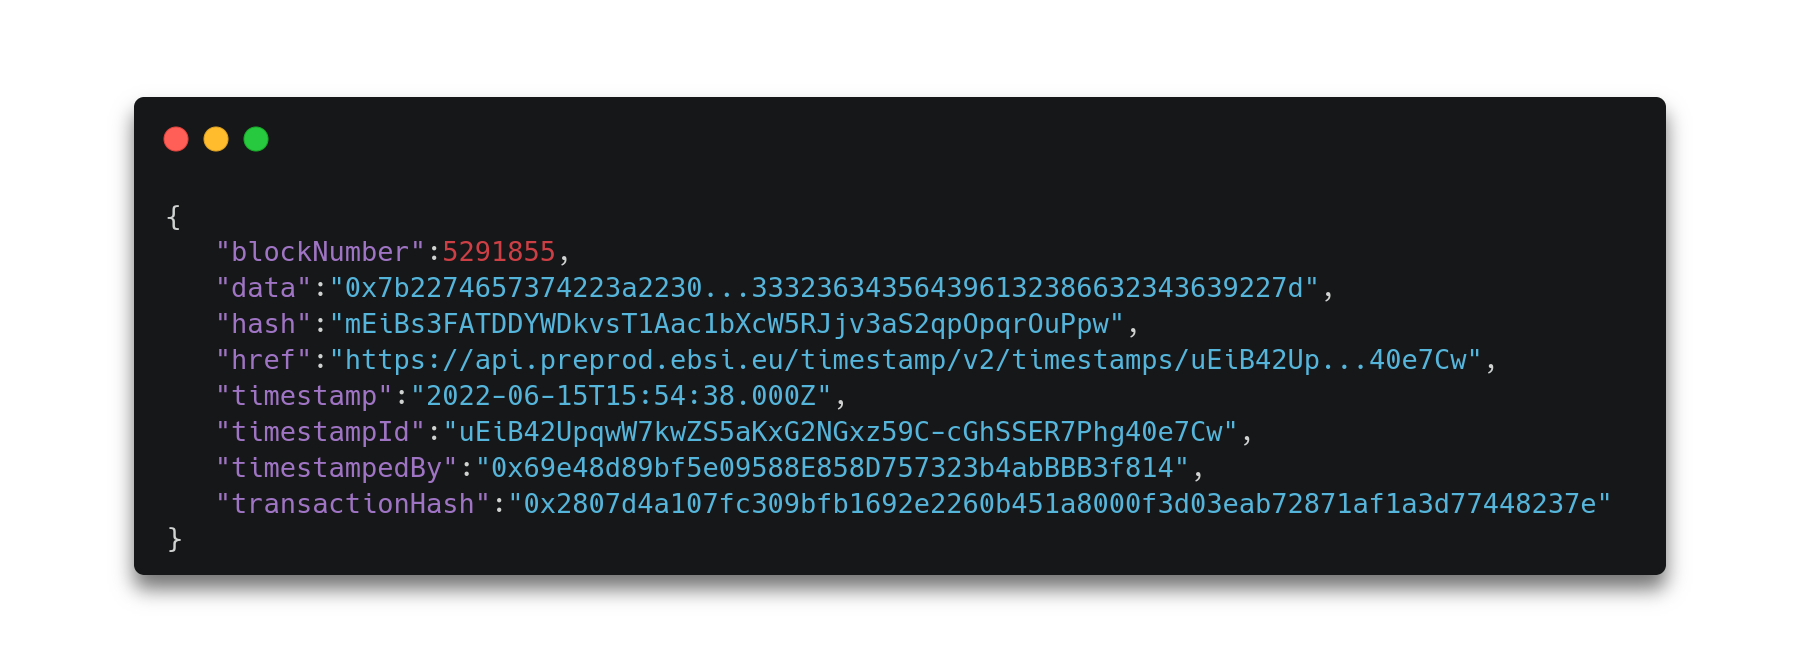
\includegraphics[scale=0.2]{chapter3/timestamp.png}
            \vspace{-0.3cm}
            \captionof{figure}{EBSI transaction timestamp example}
        \end{center}
        \vspace{0.6cm}
        \item[] \code{getTimestampByTXHash}: gets the timestamp of a specific transaction;
        \begin{itemize}
            \item \textbf{Params}: the \texttt{txHash} (\texttt{string});
            \item \textbf{Returns}: the timestamp in \texttt{JSON} format.
        \end{itemize}
    \end{itemize}

    \item \textbf{Universal Resolver}: enables the resolution of DID registered in
    other blockchains than EBSI;
    \begin{itemize}
        \item[] \code{resolveDID}: resolves a DID;
        \begin{itemize}
            \item \textbf{Params}: the \texttt{DID} (\texttt{string});
            \item \textbf{Returns}: the resolved DID in \texttt{JSON} format;
            \item \textbf{Notes}: to see the complete list of supported blockchains,
            refer to the \href{https://github.com/decentralized-identity/universal-resolver}
            {official repository}.
        \end{itemize} 
    \end{itemize}

    \item \textbf{utils.ts}: in these files can be found utilities used in the SDK, but that
    can also be used by the users, such as:
    \begin{itemize}
        \item \textbf{types}, used to enhance the readability of the code, to avoid errors and to
        make the SDK easier to use;
        \item \textbf{consts}, expecially for the API ports;
        \item \textbf{interfaces}, to define the structure of the objects used as input or
        output of the API calls, this way the user can easily understand the structure of
        the objects, and does not need to refer to the documentation each time;
        \item \textbf{functions}, such as \texttt{callAPI} (already \hyperref[fig:callAPI]
        {explained}) or \texttt{getId}, used by the SDK to get the ID of a key or DID.
    \end{itemize}
    
    \item \textbf{lib.ts}: here are placed functions that use multiple SDK methods also from
    different classes. Only two functions have been written so far, and almost only for
    testing purposes, but they can be used by the user as well, and there can be added more 
    in the future if needed.
    
\end{itemize}

\paragraph{Problems and difficulties found.}
The most challenging thing about building the SDK was understanding everything about 
the SSI Kit. The developer needed to learn everything involved in the kit: the W3C 
standards for credentials issuing and verification, the basics of cryptography,  
API interaction, and more.\\
Frequently, the API calls' input or output parameters were not specified in the 
documentation (at least, the schema was specified but not the true meaning of specific
fields). This way, the only manner to go on was to analyze the SSI Kit source code
 (this meant knowing a minimum of Kotlin) or contact the team on Slack.\\
Finally, a minor bug in the Custodian component was found during the SDK development.
It has been reported, and the team fixed it in a week.

\paragraph{Tests.}
The SDK's main components have been tested, focusing on the SSI Kit's four classes 
(Custodian, Signatory, Auditor, and ESSIF).\\
The final coverage is decent but is not 100\%, so it could be slightly improved 
by testing untested branches.t could be slightly improved by testing untested branches.\\
In the underlying images, it can be seen (in this order) all files' final coverage, 
the statements coverage, and finally branches, functions, and lines coverage details.
\vspace{0.5cm}
\begin{center}
    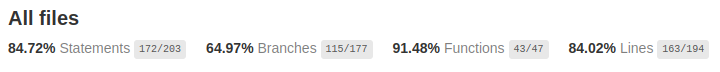
\includegraphics[scale=0.5]{chapter3/coverage1.png}
    \captionof{figure}{All files' tests coverage percentages}
\end{center}
\begin{center}
    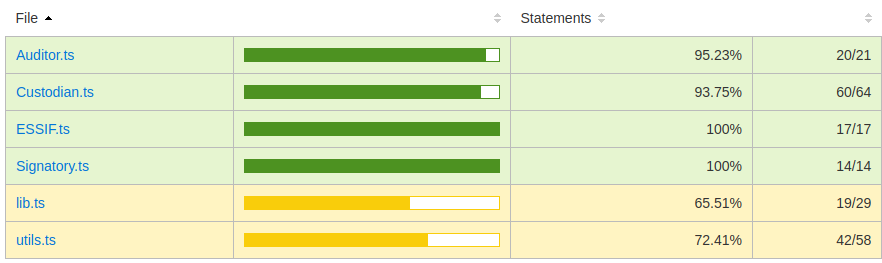
\includegraphics[scale=0.4]{chapter3/coverage2.png}
    \captionof{figure}{Visual representation and statemets coverage}
\end{center}
\begin{center}
    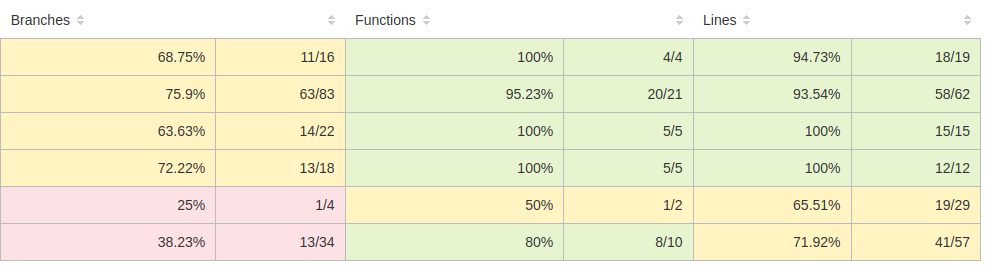
\includegraphics[scale=0.35]{chapter3/coverage3.png}
    \captionof{figure}{Branches, functions, and lines coverage details}
\end{center}

\paragraph{Documentation.}
The SDK documentation can be found at the link
\href{https://matteocasonato.gitbook.io/ssikit-sdk/}
{\seqsplit{https://matteocasonato.gitbook.io/ssikit-sdk/}}. Here can be seen the 
specifications of the SDK classes and methods and some use examples.

\subsection{Web Application Proof of Concept}
After the SDK and smart contracts development, we merged the two macro components 
into a basic web application as a proof of concept of the final solution.\\
The application serves as an interface for smart contract and SDK interaction, 
enabling users to interact with verifiable credentials.

\subsubsection{Structure}
The whole application can be divided into two main components: the frontend, which
contains the central part of the logic, thanks to React.js, and the backend, used 
just because some operations would not have been secure if done in the frontend, and 
something could not be done here because of compatibility issues (browser do not 
support all the cryptographic functions, as we explain later).

\paragraph{Frontend.}
The frontend breaks down into six main pages:
\begin{itemize}
    \item \textbf{Holder}: provides a complete interface for the SDK \texttt{Custodian}
    class; this component is divided into three sub-components:
    \begin{itemize}
        \item[] \textbf{Keys}: here the user can manage the keys used to generate
        the DIDs. The user can create a new key, export it, delete it and more;
        \item[] \textbf{DIDs}: here the user can manage their DIDs. The user can create
        a new DID, load it, delete it;
        \item[] \textbf{Credentials}: here the user can manage their credentials. The
        user can import a new credential, present it and delete it.
    \end{itemize}
    \item \textbf{Issuer}: provides a complete interface for the SDK \texttt{Signatory}
    class; this component is divided into two sub-components:
    \begin{itemize}
        \item[] \textbf{Issue}: in this component, the user can issue a credential.
        \item[] \textbf{Revocations}: in this component, the user can revoke a credential
        or check if a credential is revoked.
    \end{itemize}
    \item \textbf{Verifier}: provides a complete interface for the SDK \texttt{Auditor}
    class, and adds the on-chain functionalities for the verifiers; it is divided into 
    two sub-components:
    \begin{itemize}
        \item[] \textbf{Verifications}: here is possible to verify credentials and put the
        result on-chain as a verification record; also, verification records are searchable;
        \item[] \textbf{Verifiers}: here the smart contracts owner can add new verifiers
        and search them on-chain;
    \end{itemize}
    \item \textbf{Contracts}: on this page, the smart contracts owner can register a new
    contract as trusted or untrusted, and search them on-chain;
    \item \textbf{Diploma}: on this page, an hypothetical student can request a diploma request
    NFT, and then consume it to gain access to the final diploma certificate (VC);
    \item \textbf{EBSI}: here an user can register a DID (generated with \texttt(ebsi)
    method) on the EBSI network; serves as an interface for the SDK \texttt{ESSIF} class.
\end{itemize}
Finally, the application provides the user a web3 wallet connector, so he can interact
with the smart contracts where needed.

\paragraph{Backend.}
We needed to add a backend to our application for two important reasons:
\begin{enumerate}
    \item \textbf{Security}: the frontend is not secure enough to handle cryptographic
    operations, so we needed to move them to the backend; Specifically, when a 
    verifier wants to add a new verification record, he must create a signature with 
    the private key of its DID. The signature certificates that the real verifier is
    adding that record. As the application must interact with the user's private key, 
    this must be done at the backend level: if the private key reaches the frontend, 
    it is no longer secure. We avoided this by using the server as a REST API: when 
    it has to sign, the user passes its private key's (public) ID. The backend creates
    the signature, and it is passed to the frontend. The signature can also be 
    verified with another method.
    \item \textbf{Compatibility}: the browser does not support all the cryptographic
    functions we need. In particular, we needed the elliptic curve Secp256k1, used 
    for Ethereum accounts generation. The DID generated with the ebsi method must be 
    created with a Secp256k1 key pair because when there is an interaction with the 
    blockchain, the EBSI API will sign a message using the corresponding private key
    (which has to be compatible with an Ethereum account).\\
    Assuming this, if we use cryptographic functions from the frontend (using 
    React.js), the application will interact with the W3C Web Cryptography API. 
    Unfortunately, this API does not support the Secp256k1 curve, so we have been 
    forced to move this logic to the backend. 
\end{enumerate}

\subsubsection{Functionalities}
We now examine what the two main components of the web application, frontend, and 
backend, offer (obviously, the frontend offers functionalities to users, and the 
backend serves only the frontend).
\paragraph{Frontend.}
Now we show all the functionalities provided by each previously explained frontend's 
page.
\subparagraph{Holder.} This page is divided into three sections: \texttt{Keys}, 
\texttt{DIDs} and \texttt{Credentials}; Figure 3.9 shows the page screenshot.
\begin{center}
    \begin{tcolorbox}[
        beamer,
        width=0.6\textheight,
        arc=0pt,
        boxsep=0pt,
        left=0pt,right=0pt,top=0pt,bottom=0pt,
        ]
    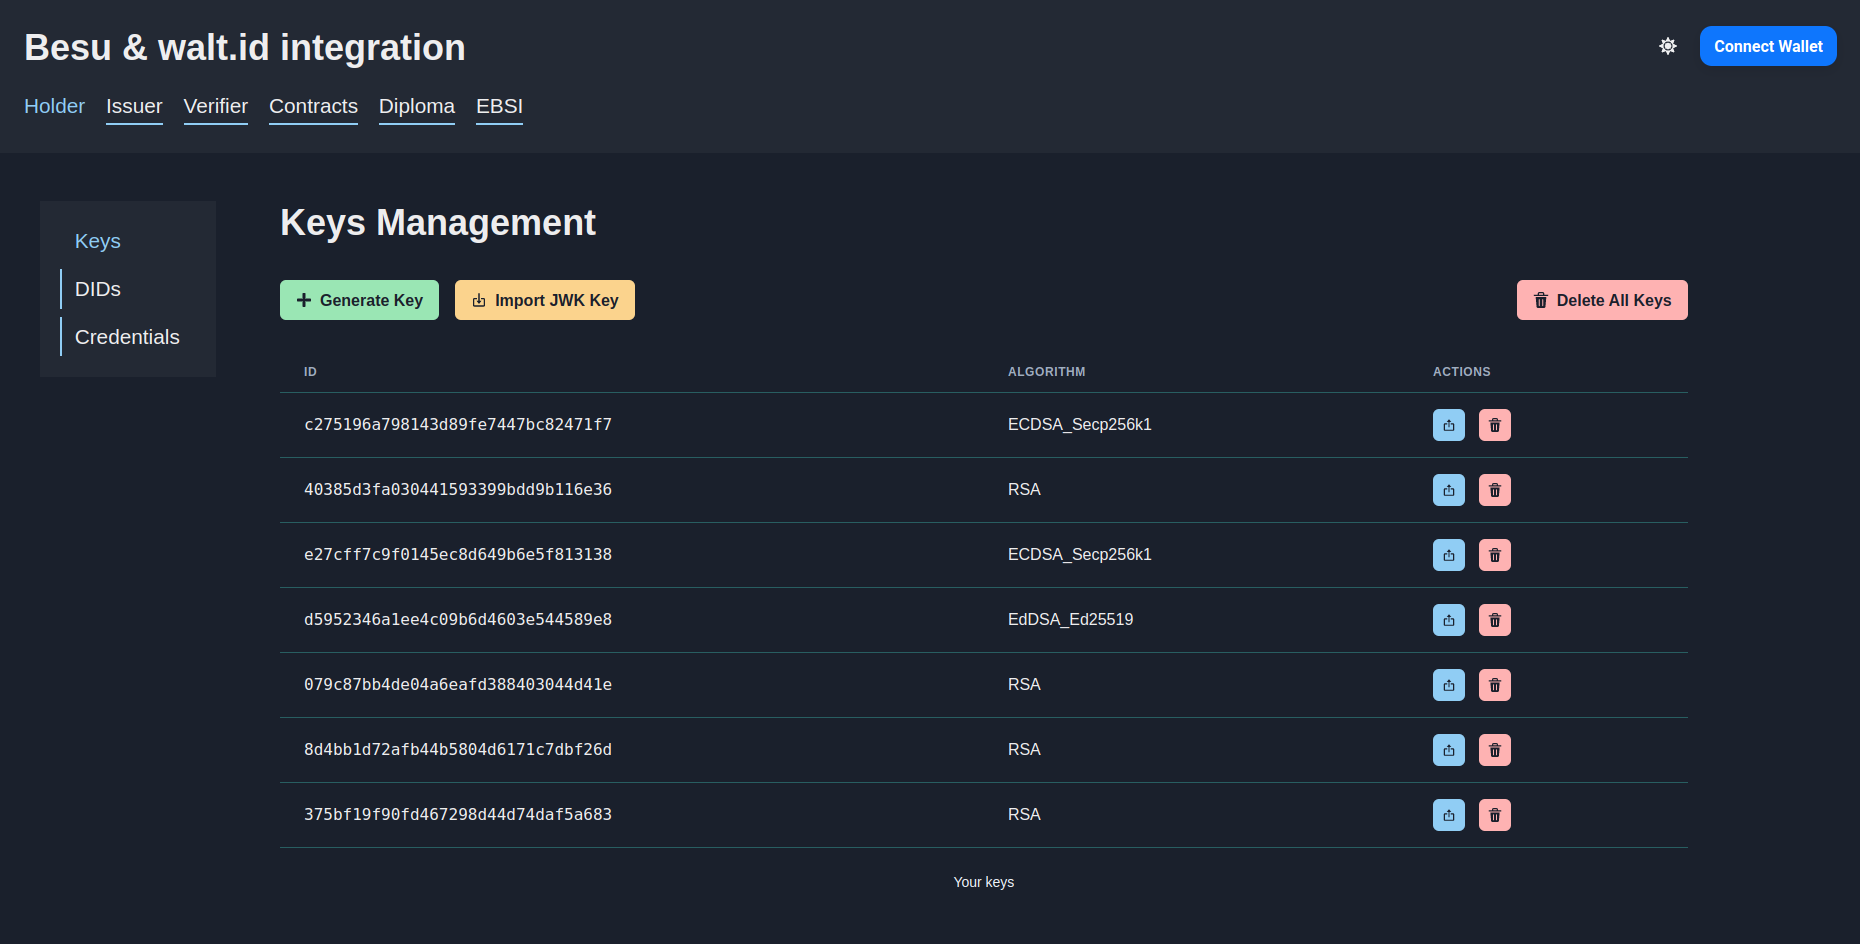
\includegraphics[width=\linewidth]{chapter3/frontend/holder.png}
    \end{tcolorbox}
    \vspace{-0.3cm}
    \captionof{figure}{The \texttt{Holder} page (\texttt{Keys} section)}
\end{center}
In the \texttt{Keys} section inside the \texttt{Holder} page, a user can:
\begin{itemize}
    \item Generate a key using a supported algorithm, by pressing the green button \texttt{Generate Key};
    \item Import a key in \texttt{JWK} format, yellow button;
    \item Export a key (public or private) in the desired format, by pressing the
    blue button;
    \item Delete a key, by pressing the red button;
    \item Delete all the keys, by pressing the red button \texttt{Delete All Keys};
\end{itemize}
\vspace*{0.3cm}
In the \texttt{DIDs} section, a user can:
\begin{itemize}
    \item Create a DID using a supported method and a previously generated key, 
    by pressing the button \texttt{Create DID};
    \item Import a DID inserting its string, by pressing the button \texttt{Import DID};
    \item Resolve a DID by pressing the button \texttt{Resolve DID} (remembering that
    \texttt{did:key} are in local, and \texttt{did:ebsi} are resolved from the blockchain);
    \item View a DID loading it from the local storage by pressing the button in the table;
    \item Delete a DID (from local storage) by pressing the button in the table;
    \item Delete all the DIDs, by pressing the button \texttt{Delete All DIDs};
\end{itemize}
\vspace*{0.3cm}
In the \texttt{Credentials} section, a user can:
\begin{itemize}
    \item Import a credential, giving it an alias, by pressing the button \texttt{Import Credential};
    \item Present one or more credentials, selecting them in the credentials table
    and by pressing the button \texttt{Present Credential};
    \item View a credential loading it from the local storage by pressing the button in the table;
    \item Delete a credential by pressing the button in the table;
    \item Delete all the credentials, by pressing the button \texttt{Delete All Credentials};
\end{itemize}

\clearpage
\subparagraph{Issuer.} This page is divided into two sections: \texttt{Issue}
and \texttt{Revocations}; Figure 3.10 shows the page screenshot.
\begin{center}
    \begin{tcolorbox}[
        beamer,
        width=0.6\textheight,
        arc=0pt,
        boxsep=0pt,
        left=0pt,right=0pt,top=0pt,bottom=0pt,
        ]
    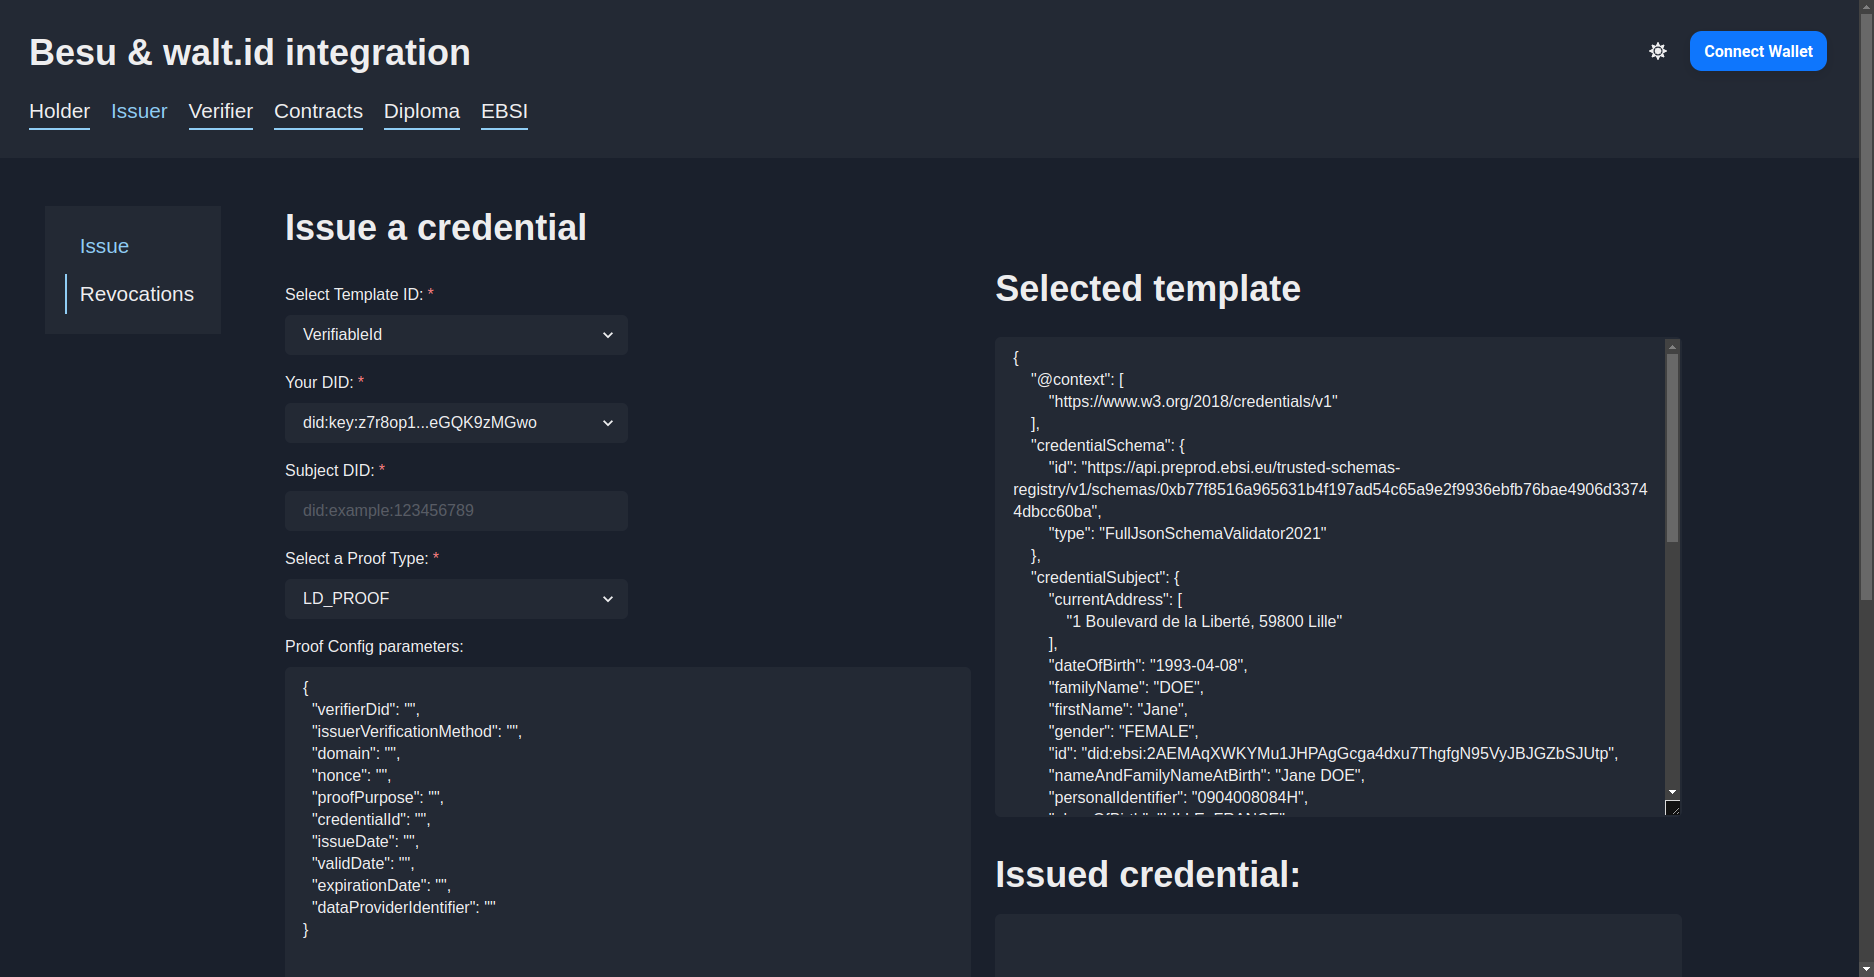
\includegraphics[width=\linewidth]{chapter3/frontend/issuer.png}
    \end{tcolorbox}
    \captionof{figure}{The \texttt{Issuer} page (\texttt{Issue} section)}
\end{center}
In the \texttt{Issue} section, an issuer can issue a credential by filling out the form and
by pressing the button \texttt{Issue Credential}. First, he must select a template,
used for the generation. Then, he must configure the credential, with the possibility
of adding optional fields. The credential is then generated
and inserted in the \texttt{Issued credential} field, and we can copy that and import
locally the issued VC in the \texttt{Holder} page. In a real use case, the credential
would be sent to the holder using secure communication protocols such as \texttt{OIDC}.
\vspace*{0.3cm}\\
In the \texttt{Revocations} section, an issuer can revoke a credential by inserting
the corresponding private revocation token he generated when he issued the credential.
The revocation is off-chain, and we have not yet implemented the on-chain call (from the
frontend) that would change the verification record (however, the function is
implemented in the smart contract). Also, anyone can check if the credential has been
revoked by inserting the corresponding public revocation token.

\clearpage
\subparagraph{Verifier.} This page is divided into two sections: \texttt{Verifications}
and \texttt{Verifiers}; Figure 3.11 shows the page screenshot.
\begin{center}
    \begin{tcolorbox}[
        beamer,
        width=0.6\textheight,
        arc=0pt,
        boxsep=0pt,
        left=0pt,right=0pt,top=0pt,bottom=0pt,
        ]
    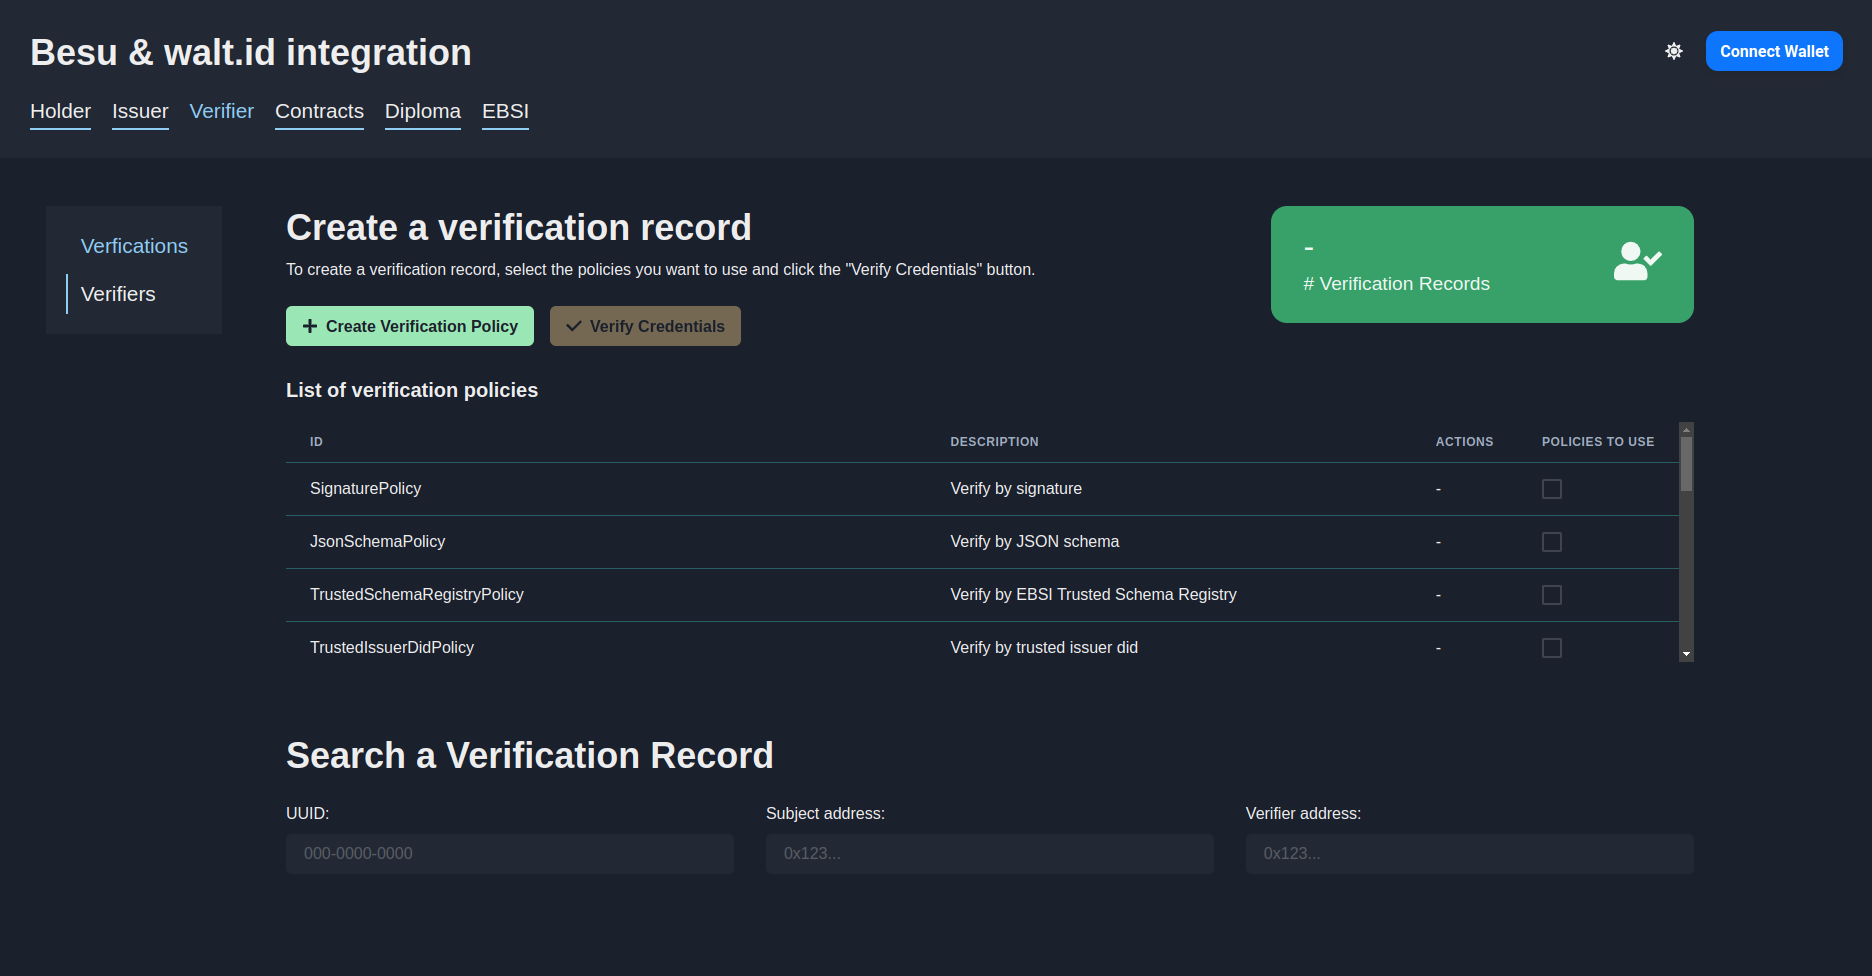
\includegraphics[width=\linewidth]{chapter3/frontend/verifier.png}
    \end{tcolorbox}
    \captionof{figure}{The \texttt{Verifier} page (\texttt{Verifications} section)}
\end{center}
\vspace{0.3cm}
In the \texttt{Verifications} section, a verifier can:
\begin{itemize}
    \item Create a verification policy by pressing the green button;
    \item Verify a credential and register the result on-chain as a verification record. 
    To do so, he must select at least a verification policy from the list.
    Before adding the result on-chain, the verifier creates a signature with the 
    private key of its DID. This way, anyone can resolve their DID and use the public 
    key (findable in the credential's \texttt{verificationMethod} field) to verify the 
    signature;
    \item Search for an on-chain verification record.
\end{itemize}
\vspace*{0.3cm}
In the \texttt{Verifiers} section, the contract owner can register on-chain a new 
verifier, adding it to the trusted verifiers' list. Anyone here can see the list of
trusted verifiers and search for a specific one.
Here is where we manage to merge the off-chain and on-chain solutions in
the PoC. Other functionalities can be added (e.g., on-chain revocation after off-chain
happened), but for time reasons, we have only implemented the verification record 
registration.

\clearpage
\subparagraph{Contracts.} Figure 3.12 shows the page screenshot.
\begin{center}
    \begin{tcolorbox}[
        beamer,
        width=0.6\textheight,
        arc=0pt,
        boxsep=0pt,
        left=0pt,right=0pt,top=0pt,bottom=0pt,
        ]
    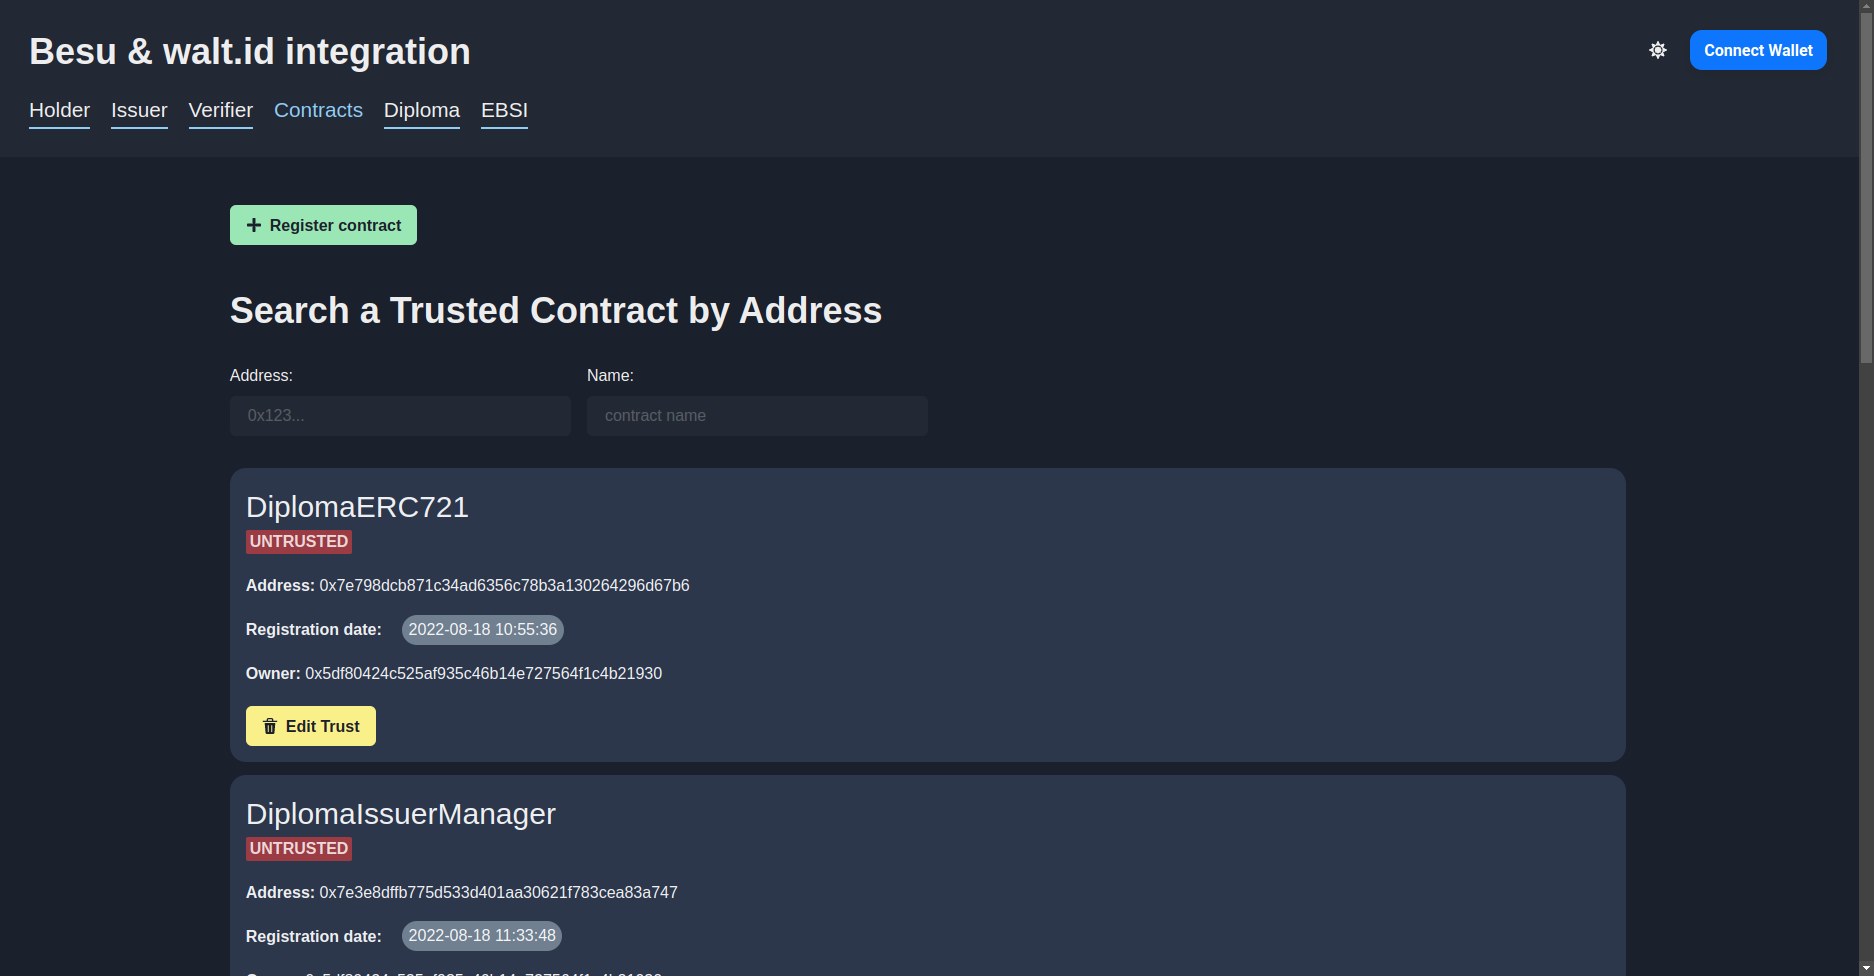
\includegraphics[width=\linewidth]{chapter3/frontend/contracts.png}
    \end{tcolorbox}
    \captionof{figure}{The \texttt{Contracts} page}
\end{center}
On this page, the contract owner can register a contract as trusted or untrusted
in the on-chain list. Anyone can see the list of contracts and search for
a specific one.

\vspace{1cm}
\subparagraph{Diploma.} Figure 3.13 shows the page screenshot.
\begin{center}
    \begin{tcolorbox}[
        beamer,
        width=0.6\textheight,
        arc=0pt,
        boxsep=0pt,
        left=0pt,right=0pt,top=0pt,bottom=0pt,
        ]
    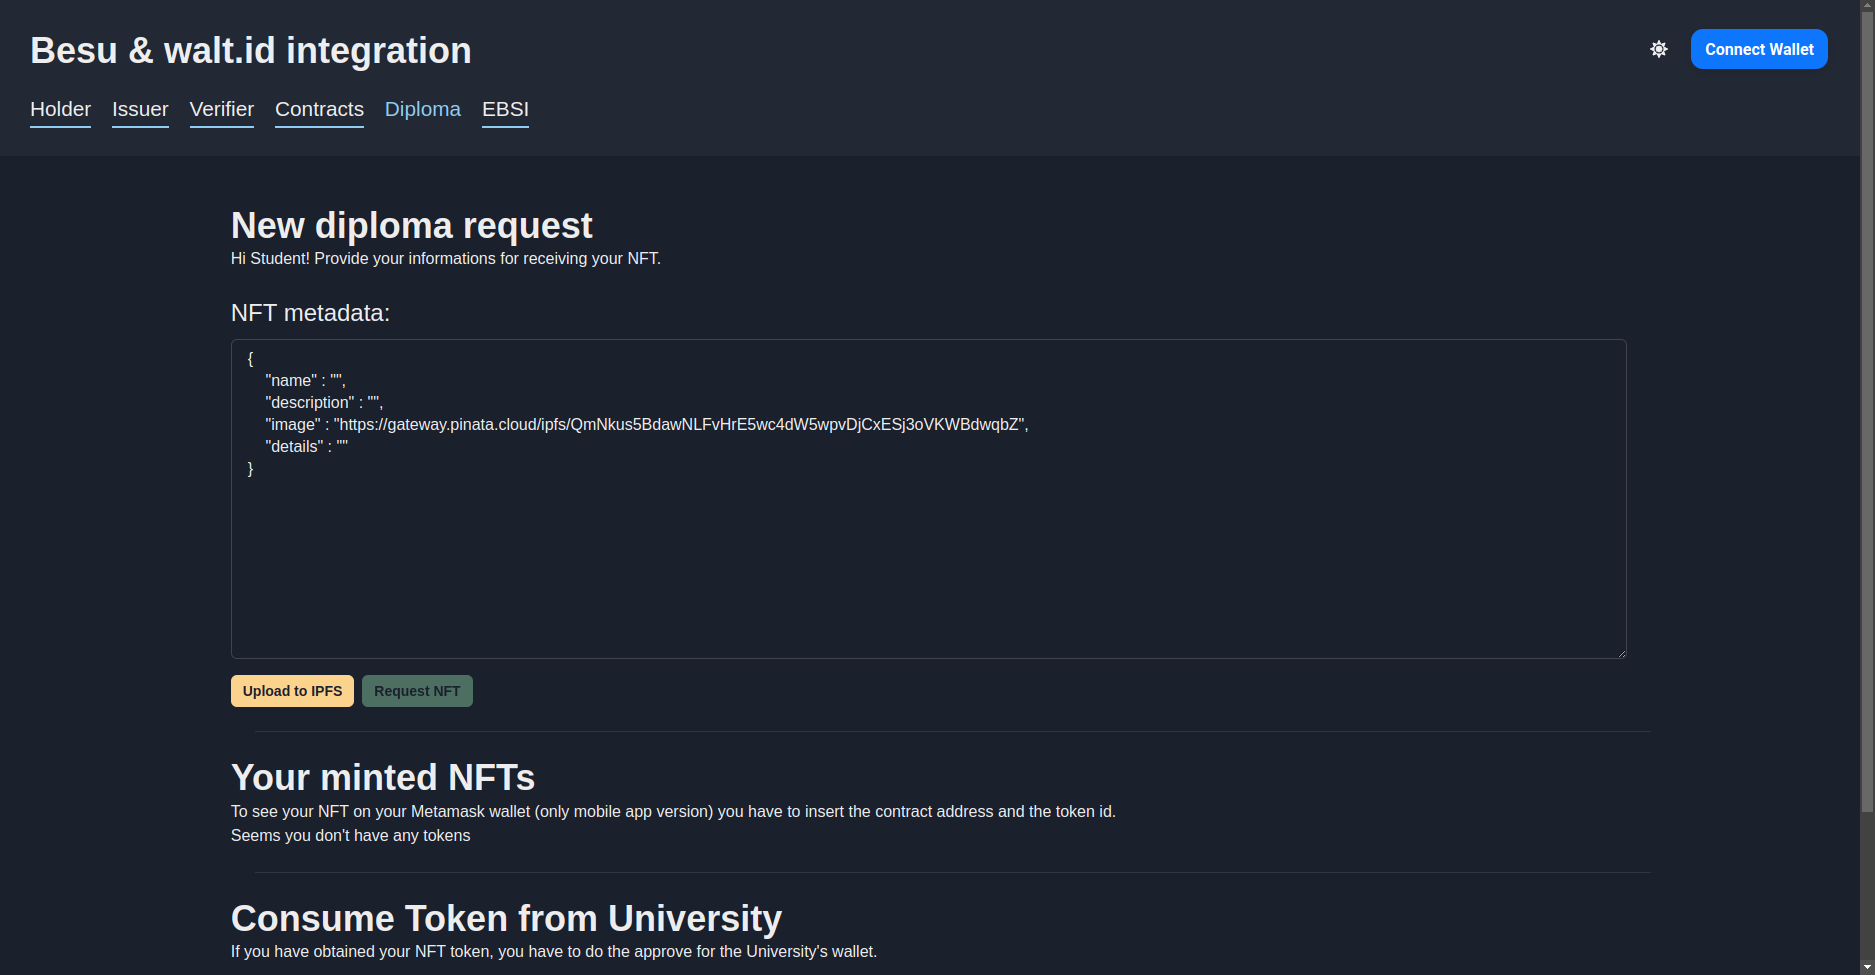
\includegraphics[width=\linewidth]{chapter3/frontend/diploma.png}
    \end{tcolorbox}
    \captionof{figure}{The \texttt{Diploma} page}
\end{center}
\clearpage
On this page\footnote{The details of this whole operation are not explained in this paper,
as they are examination subjects of another student's thesis.}:
\begin{itemize}
    \item A student can request an NFT usable by the user to officially request the diploma;
    \item The university sees all the NFT requests and can accept them by minting
    the Request NFT to the student's wallet;
    \item A student can approve the university to burn the Request NFT; after that,
    the university can consume (or burn) the Request NFT and issue the VC diploma to 
    the student (issuing procedure is not implemented).
\end{itemize}

\vspace{1cm}
\subparagraph{EBSI.} Figure 3.14 shows the page screenshot.
\begin{center}
    \begin{tcolorbox}[
        beamer,
        width=0.6\textheight,
        arc=0pt,
        boxsep=0pt,
        left=0pt,right=0pt,top=0pt,bottom=0pt,
        ]
    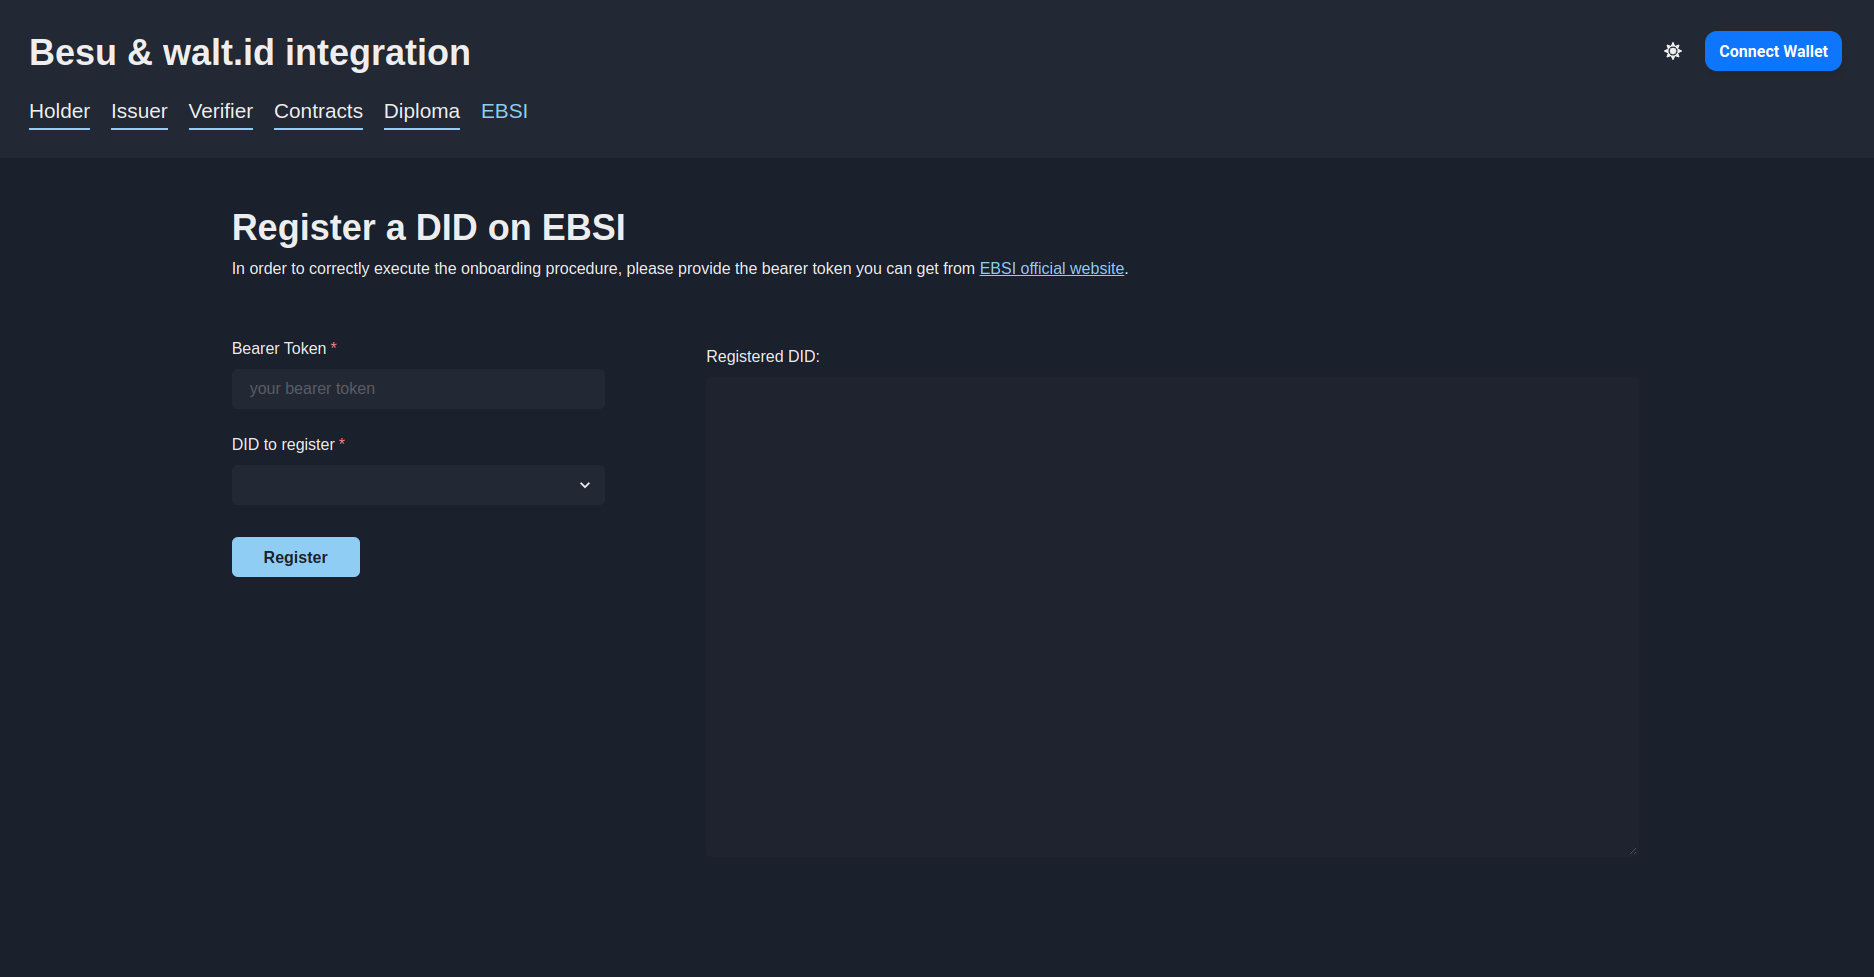
\includegraphics[width=\linewidth]{chapter3/frontend/ebsi.png}
    \end{tcolorbox}
    \captionof{figure}{The \texttt{EBSI} page}
\end{center}
\vspace{0.3cm}
A user can register a DID on the EBSI network on this page. The user must insert
the \texttt{bearerToken}, obtainable on the EBSI official website. The interface
simplifies the registration process: as explained in the SDK section,
the process needs three steps, but the user sees only one.

\clearpage
\paragraph{Backend.}
The backend is designed as a REST API. We used it to implement the creation 
and verification of the signatures made by the verifiers when they register 
on-chain a verification record.
\vspace{0.3cm}\\
The functions made available to the frontend are two:
\begin{itemize}
    \item \code{/createSignature}: the verifier signs the verification record
    with its DID private key. In the request body, the verifier must insert the
    \texttt{JSON signatureRequest object}, which has two fields: \texttt{keyId},
    where is specified the private key (public) ID, and \texttt{message},
    which is the message to sign (in this case, the verification record);
    the call response is the signature in \texttt{JWS} format;
    \item \code{/verifySignature}: any user (from the frontend, if the
    interface is implemented) can verify a signature. In the request body, the
    verifier must insert the \texttt{JSON verificationRequest object}, which has
    three fields: \texttt{verifierDid}, where specified the DID of the
    verifier who signed the message, and \texttt{message}, which is the
    message to verify (also in this case, the verification record: if the
    verification record data coincides with the decoded signature payload,
    then the signature is valid and the verification record is valid too);
    if the signature is valid, the call response is the signature payload (which
    should be equal to the verification record), otherwise the function
    will throw an error.
\end{itemize}

\subsubsection{Problems and difficulties found}
Generally, we have not found crucial problems during the PoC development. The only 
difficulty was the signature creation; it took a while to find the real 
problem (i.e., the \texttt{Secp256k1} curve incompatibility with the W3C Web 
Cryptography API). Also, we had to compromise: verifiers, to generate the signature, 
can only use DID created with the \texttt{ebsi} method (so also with \texttt{Secp256k1}
curve). The \texttt{/verifySignature} has to be revisited to enhance interoperability
with other methods and encryption algorithms.

\section{Discussion}
In this last section, we discuss the last considerations about the final result, what 
can be done to improve the solution, and some personal thoughts.

\subsection{Achievements}
We partially merged the off-chain and on-chain solutions. The verifier integration works well,
also from a security point of view, thanks to the signatures implementation.\\
Thanks to the existing standards (which are in development), we created a system where 
users can own their credentials. We created an SDK that simplifies the interaction with 
SSI primitives, a smart contract suite that reflects on-chain the off-chain events, and 
the proof of concept web application gives an idea of what a user can do with the final 
solution.
So objectively, we reached a satisfying grade of requirements fulfillment, as initially
we were not sure about the possibilities.

\subsection{Future developments}
It is obvious to remark that we are only at the beginning of SSI solutions development. 
Standards are being defined now, and developers do not know the right path to pursue 
since it is an exploration.
There can be many future developments for these solutions and the SSI model, especially
for seamless integration with permissionless blockchains. Let us divide them into two 
categories: PoC improvements and SSI next challenges.
\subsubsection{PoC improvements}
Some of the possible PoC improvements are:
\begin{itemize}
    \item \textbf{Revocations}: they could be forced to be instantly reflected on-chain
    with a smart contract call after the revocation is made on the off-chain side, as
    is already done for verifications;
    \item \textbf{Diploma issuance}: when a user consumes the Request NFT, the university
    should be able to see it from the frontend and issue the diploma in a guided and
    easier way provided by the \texttt{Issuer} page;
    \item \textbf{Issuer}: the \texttt{Issue} section could be significantly improved from
    a UX perspective, as it is now a basic form, easy to use just for a developer who
    knows what he is doing;
    \item \textbf{Secure communication protocols}: a thing that we did not implement is the
    secure verifiable credential exchange. Fortunately, walt.id kits provide API to
    implement this feature, so it is possible to add it in the future also using those kits;
    \item \textbf{On-chain DID signature check}: it could be helpful to move the signature 
    verification (now provided by the frontend through \code{/verifySignature}) to the 
    smart contract level when a verification record is being created;
    in this way, the transaction could be reverted if the signature is not valid (i.e., 
    the verifier is not signing with the DID private key), and no one should check if 
    the signature is valid as if it is on-chain it is valid;
    \item \textbf{Sign with new DID methods}: currently, the only DID method supported 
    for the signature creation, and so for the verifiers' functions, is \texttt{ebsi}; 
    at least should be added the \texttt{key} method, to enhance the product usability.
    \item \textbf{New DID methods}: New DID methods should be added to widen the entire 
    product's interoperability. An easy way to do this should be searching for already 
    existing SDKs (if not in Typescript/Javascript, then they should be wrapped as the 
    SSI Kit SDK) that support different blockchains (e.g., MATTR and Veramo, explained
    in \hyperref[otherSDKs]{Chapter 2}) and integrating them in the PoC. Also could be 
    interesting to add a new wrapper level that includes all the wrappers, as Figure 
    3.15 shows.
    \begin{center}
        \hspace{-1cm}
        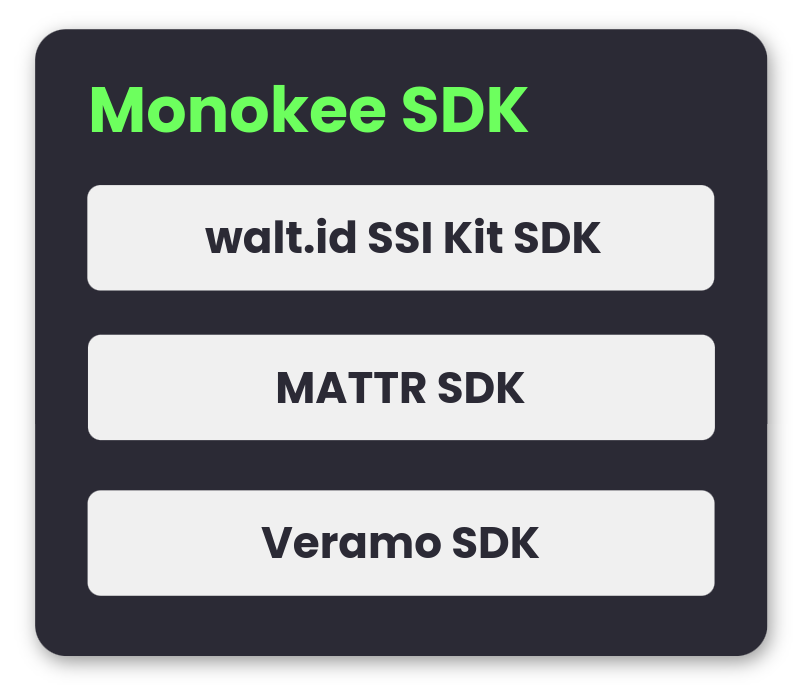
\includegraphics[scale=0.28]{chapter3/monokeesdk.png}
        \vspace{-0.3cm}
        \captionof{figure}{Monokee SDK could wrap other SDKs to enhance interoperability
        with different blockchains.}
    \end{center}
\end{itemize}
\subsubsection{SSI next challenges}
Developing the whole product, we studied the SSI model and its primitives. By the way, 
Self-Sovereign Identity is far from ready for actual adoption. Standards are under 
development, but this technology has enormous potential for sure.\\
In \hyperref[subsubsec:comparison]{Chapter 2}, we made a comparison between permissionless
and permissioned blockchains. For the time being, a significant part of SSI technologies
works with permissioned blockchains because it is easier to preserve privacy, as here 
transactions are encrypted, and networks are accessible to trusted members. In 
permissioned blockchains, the model seems can work. They fit well in federated and 
private environments where trust is needed and welcome (for example, in a private company). However, what when we talk about 
public environments? Trust is also needed here, but let us consider this scenario: EBSI 
is a federated blockchain with public purposes. What happens if the majority of the nodes 
ally to attack the network? Or if it gets hacked? Is this considered impossible? Why 
should people trust the authorities when the network works by design, and people do not need
to trust it? Attacking a network of few nodes (about thirty) is more effortless than 
attacking, for example, Ethereum (a permissionless blockchain), which has more than 
420.000 validators. So, if Self-Sovereign Identity wants to give back users their data, 
it should not force them to trust other entities.\\
One of the main problems with bringing SSI on-chain is privacy preservation. Everything is public (unless encrypted) 
on permissionless blockchains, making moving every SSI primitive on-chain challenging. A 
VC is off-chain because it is easier to keep private, and moving it on-chain without proper 
encryption mechanisms would destroy privacy. This is not a trivial problem, and 
researchers are trying to solve it. The latest proposals are ERC-725 standard, zkKYC
and soulbound tokens.

\paragraph{ERC-725.} It is a proposed standard for blockchain-based identity authored by Fabian 
Vogelsteller, creator of ERC-20 and Web3.js. ERC-725 describes proxy smart contracts that 
can be controlled by multiple keys and other smart contracts. ERC-735 is an associated 
standard to add and remove claims to an ERC-725 identity smart contract. These identity 
smart contracts can describe humans, groups, objects, and machines. ERC-725 lives on the
Ethereum blockchain.

\paragraph{zkKYC} Know Your Customer (KYC) is a process that is used to verify the identity 
of a user. It is a crucial step in the onboarding process of a user in a financial 
institution, for example in a bank or a crypto exchange. The problem is that KYC is a 
centralized process, and the user has to trust the institution that is asking for his
data. zkKYC is a proposal that uses zero-knowledge proofs to verify the identity of a user
without revealing all of his data.

\paragraph{Soulbound tokens} They essentially are non-transferable NFTs (this is the name 
reason). In this way, a municipality could mint for a citizen his ID as a soulbound NFT, 
and the citizen could use it to prove his identity. The token is non-transferable, so it 
cannot be stolen or used by someone else. The problem is that the token is on-chain, and 
so it is public. To preserve privacy, Vitalik Buterin propose some solutions in his blog 
post "Soulbound". One of them, is using zkSNARKs to prove something related to the 
soulbound token.
\\\\
As is understandable, zero-knowledge proofs will play an essential role in SSI progress, 
and we are just at the beginning of the development. These are just some examples that try to solve the 
biggest SSI problems, and as it is understandable, there is still much work to be done.

\subsection{Personal evaluation}
On the technical side, I think we have done a great job. Initially, it was tough to 
understand what we had to do, as we were helping the team understand it. The path became 
evident when we completely understood SSI and what the team wanted to do with the product.
I am proud of the job we have done and the achievement we have reached.\\
I am glad I chose such a project to develop because it seeks to solve current fundamental
problems. I am deeply interested in web3, and before this project, I had read about 
Self-Sovereign Identity but never studied and understood its concepts and components so 
in-depth.\\
Now I firmly believe this needs to be part of our future, and fortunately, many researchers 
and developers are building the foundations. Monokee's team is part of them, and I believe 
that their product could play a key role in the SSI landscape as, in many circumstances, 
a hybrid solution is the best solution.\\

%**************************************************************
% Materiale finale
%**************************************************************
\backmatter
\chapter*{Conclusion}
Taking up what was said in the abstract, we can confirm that the final product embraces 
SSI concepts and tries to take it to the next level with the help of smart contracts.  
The developed SDK enables the issuers to release Verifiable Credentials to holders who 
own them and present them to verifiers who can confirm their validity. Thanks to smart 
contracts, we can register on-chain verification results to make them public and speed 
up the following verifications. The final proof of concept proves that off-chain SSI 
primitives can be reflected on-chain. To do so, compromises are needed to preserve 
privacy (e.g., using a permissioned blockchain as VDR simplifies things).
\vspace{0.3cm}\\
Our final product leaves room for numerous additional features, meaning that this was 
not thought of as definitive software but as a beginning for the following implementations.
We are confident that Self-Sovereign Identity will catch on sooner or later, and the 
conclusive result of this thesis offers just a taste of what these innovative and
promising technologies could bring.
\printglossary[type=\acronymtype, title=Acronimi e abbreviazioni, toctitle=Acronimi e abbreviazioni]
\printglossary[type=main, title=Glossary, toctitle=Glossary]
% !TEX encoding = UTF-8
% !TEX TS-program = pdflatex
% !TEX root = ../thesis.tex

%**************************************************************
% Bibliografia
%**************************************************************
\cleardoublepage
\chapter{Bibliography}
\nocite{*}

% Stampa i riferimenti bibliografici
\printbibliography[
    heading=subbibliography,
    title={Bibliographical references},
    type=article,
]

% Stampa i siti web consultati
\printbibliography[
    heading=subbibliography,
    title={Websites consulted},
    type=online,
]

\end{document}
